\chapter{Wave climate on the southeastern Wisconsin coast of Lake Michigan: Perspective from wave systems}
\label{chapter4}

\section{Introduction}
\label{c4_Introduction}

Wave climate, which refers to characteristics of wave conditions
\citep{wiegel_oceanographical_2013}, is an important concept in coastal oceanic
areas as it plays a significant role across various aspects including
engineering, and geomorphological change and ecology. Key wave climate
parameters, such as wave height, wave period, and wave energy, are widely
applied in coastal and oceanic engineering. These parameters are essential for
various applications including navigation safety design
\citep{lee_boundary_2009,phelps_ship_1995}, ship responses
\citep{phelps_ship_1995}, inner harbor design
\citep{romano-moreno_multimodal_2023}, energy facility development
\citep{lee_boundary_2009,liu_wind_2017} , and breakwater-wave interaction
\citep{jiang_wave_2017,lee_comparison_2006}. In addition, wave climate plays a
crucial role in shaping and controlling the evolution of coastal morphology. For
example, wave climate can drive nearshore sediment transport, which causes
severe beach erosion and bluff failure
\citep{benumof_relationship_2000,brown_factors_2005,lamoe_wave_1989}. Beach
erosion and bluff failure are two coastal hazards which is able to pose
substantial losses to coastal communities, infrastructure, and local economies.
Last but not least, wave climate can impact the health of coastal natural
habitats \citep{meadows_cumulative_2005}. In the Great Lakes, lake trout, an
economically significant species, often spawn in areas with high wave-induced
turbulence.  This turbulence, driven by high speeds wave climate, plays a
crucial role in enhancing oxygen dissolution in the water and preventing egg
smothering by fine sediments
\citep{fitzsimons_relationship_2014,sly_interstitial_1988}. In summary, wave
climate plays a vital role in coastal and oceanic environments for its
significant impacts on engineering structures, coastal morphology, and natural
ecosystems.

Wave systems climate is a characteristic of wave energy using directional wave
energy spectrum. Conventional wave climate analysis primarily focuses on key
wave statistics, such as wave height and wave period. Nevertheless, this
approach can sometimes be limited in scope, as it overlooks the directional
distribution of wave energy, which is essential for understanding complex
coastal and oceanic processes. Wave system can address this limitation by
employing wave spectrum partitioning techniques that splits wave spectrum into
distinct components, which corresponds to their original meteorological events
\citep{jiang_wave_2019,portilla-yandun_wave_2015}. This provides valuable
insights into states and directionality of wind-waves, which refer to the
combination of locally generated wind waves and swells arriving from distant
sources at a specific direction \citep{han_directional_2022}. Local wind-sea
waves typically refer to waves with short periods, as they are associated with
immature and irregular ripples driven by local wind forces
\citep{hanson_wind_1999}.  In contrast, swell waves are fully developed waves
that have propagated over long distances from their generation area, often
originating from distant storms or weather systems \citep{alford_internal_2001}.
In the directional wave spectrum, the energy of swells is generally concentrated
in the low-frequency region, while the energy of wind-sea waves usually occupies
in the higher frequency region, reflecting their difference in terms of wave
length and speed \citep{george_nearshore_2020,vettor_global_2020}.
Understanding directionality and states of the wind-waves (swell or wind-sea) is
crucial for characterizing directional spectral wave climates, as the states and
directionalities of wind waves can result in distinct physical implications,
particularly for nearshore sediment transport \citep{george_nearshore_2020}.
Wind-sea waves, with their shorter periods and higher frequencies, are more
effective at stirring and mobilizing sediment in shallow waters due to their
steepness and higher orbital velocities near the seabed
\citep{boechat_albernaz_effects_2019,nabavianpour_experimental_2024}. In
contrast, swell waves, with their longer periods and lower frequencies, can
transport sediment over longer distances and contribute to broader-scale coastal
reshaping \citep{basaran_effect_2021}.  Moreover, in some cases, opposing
directionality of sediment transport from wind waves and swells can result in
imbalances of sediment budget, leading to dramatic coastal changes
\citep{hapke_review_2010}. To date, directional spectral wave climate provides a
wider insight on the directionality and states of wind waves.

Wave systems partitioning is a crucial technique for characterizing the wave
climate from spectral data, as it allows the decomposition of the swells
generated by distant storms or wind-sea driven by local wind forcing
\citep{jiang_wave_2019,portilla-yandun_wave_2015}. The wave system partitions
can be divided into two key steps: partitioning for separating spectrum into
independent areas and classifying for aligning the area into corresponding sea
state. For the first step, the partitioning algorithms can be broadly classified
into two main categories based on the dimensions of the wave spectrum they
analyze: one-dimensional and two-dimensional algorithms
\citep{portilla_spectral_2009}.  One-dimensional partitioning algorithm
disregards wave directionality and instead differentiates different wave systems
by applying frequency-based criteria for decomposition. For example, a common
one-dimensional partition algorithm is spectrum peak method, where each local
peak of energy spectrum will be identified as an independent peak of wave system
\citep{portilla_spectral_2009,violante-carvalho_growth_2001,voorrips_assimilation_1997}.
The primary limitation of one-dimensional partitioning is its inability to
account for the directionality of different sub partitions, as these two
components often exhibit differing directional characteristics
\citep{george_nearshore_2020}.  Two-dimensional wave spectrum partition could
partition wind-sea and swell in direction-frequency domain by adding the
information of wind speed and wind direction. The first 2-d partition algorithm
was proposed by Gerling in 1992, where the algorithm detects the connectivity of
all sub-partitions over a minimum energy threshold
\citep{gerling_partitioning_1992}. Subsequently, a novel approach—the watershed
algorithm—was introduced for spectrum partitioning. This method reduces the
dependency on spectrum availability \citep{hasselmann_improved_1996} and offers
an adjustable parameter \citep{hanson_automated_2001}.
\citet{portilla_spectral_2009} further refined this approach by incorporating a
convolution kernel to smooth out spurious partitions, improving the accuracy and
reliability of the spectral decomposition. For the second step, the common
approaches of swell/wind-sea classification are introduced by
\citet{komen_existence_1984} and \citet{jensen_lake_2012}, which classify the
wind-sea and swell y comparing wave speed with wind speed. To the best of the
author's knowledge, these identification approaches are applied to NDBC
(National Data Buoy Center) data and WIS (Wave Information Study) data, which
represent two primary sources of measured and hindcast wave data in Lake
Michigan, respectively. In summary, two-dimensional wave system partitioning
allows for the extraction of both directional and spectral information from the
wave spectrum, enabling a detailed characterization of the directional spectral
wave climate.

Numerous previous studies have utilized wave system partitioning to investigate
wave climatology in oceanic and coastal environments. The first study to apply
wave spectrum analysis to wave climate research was conducted by
\citet{hanson_automated_2001}, where they presented a systematic workflow
encompassing spectral partitioning, swell tracking, and source storm
identification over a series of spectra data in Gulf of Alaska. However, this
approach requires tracking the swell event across the spectra in different
timestamps, which is sometimes hard to implement. To reduce the complexity,
\citet{portilla-yandun_wave_2015,portilla-yandun_climate_2016} further advanced
this approach by introducing an occurrence map to illustrate the statistical
distribution of local wind-sea and remote swell in Pacific Ocean. With these
approaches, wave spectral analysis has since been applied extensively to
characterize wave climates across various spatial and temporal scales. Studies
have explored regional wave climates, such as those in local scales
\citep{romano-moreno_multimodal_2023,venolia_historical_2024,zheng_investigation_2024}
and the oceanic scale
\citep{jiang_wave_2019,langodan_unraveling_2018,portilla-yandun_climate_2016}
even global scales \citep{echevarria_seasonal_2019,echevarria_influence_2020}.
Despite the well-established applicability of wave spectrum analysis in oceanic
environments, the directional spectral wave climate of Lake Michigan remains
relatively understudied. Compared to oceanic climate, Lake Michigan exhibits a
similar wave climate characterized by both strong bimodality and
bidirectionality of sea states. Nevertheless, Lake Michigan also exhibits a
distinct wave climate characterized by relatively minimal tidal ranges and
limited fetch field, making it challenging to directly apply findings from
oceanic studies to this freshwater lake system. These unique features
necessitate a detailed investigation using wave system partitioning techniques
which applied in oceanic areas, serving as the primary motivation for this
study.

\textcolor{red}{Need to rewrite}

The objective of this chapter is to characterize the climate of wave systems in
Lake Michigan by wave spectrum partitioning. To archive this, the directional
energy spectrum will be contructed using NDBC data from the 2011 to 2023. Wave
system partitioning will be applied to the spectra in the offshore of Lake
Michigan buoys (NDBC) to obtain wave systems (wind-sea and swell). The results
of wave system partions will be validated with the Wave Information Study (WIS)
partitions to select the most appropriate partitions hyper-parameters. With the
wave system partitions, the climatology of the wave systems will be further
characterized and studied, including the directional distributions of
significant wave height ($H_s$). The annual and monthly patterns of the wave
system is also reported. 
\section{Study site}
\label{c4_study_site}

\begin{figure}[htbp]
  \centering
  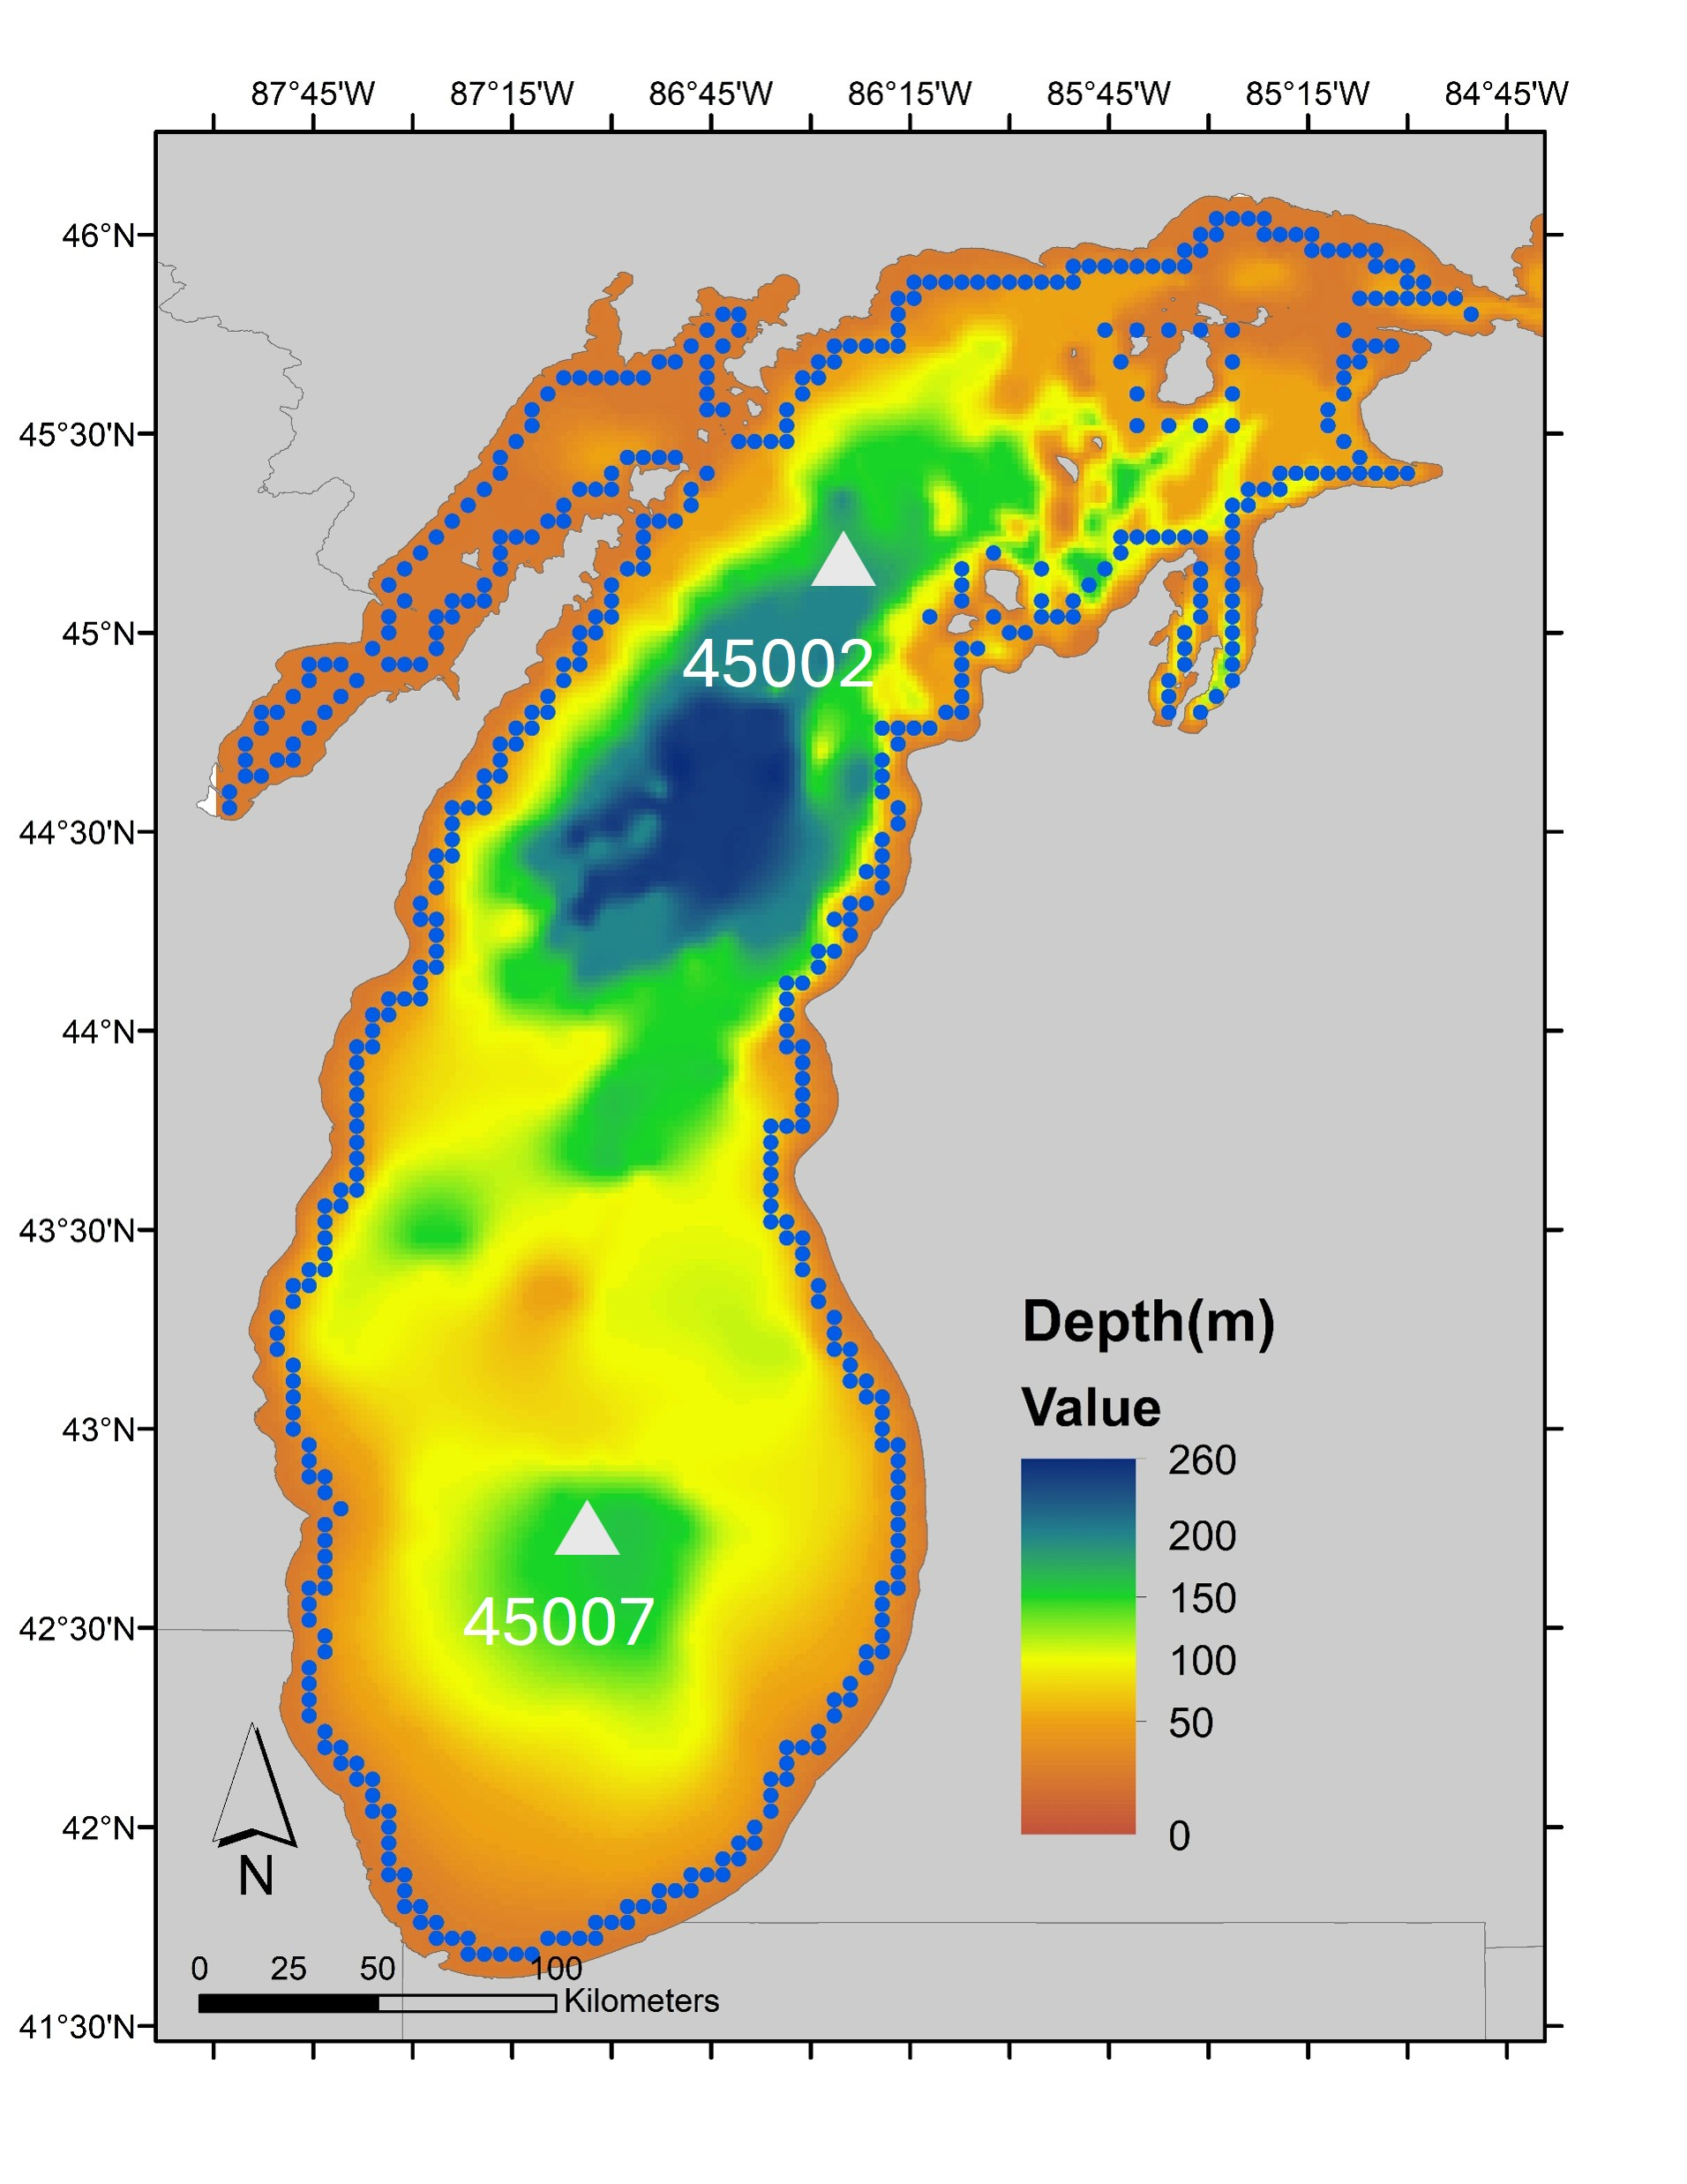
\includegraphics[width=0.8\textwidth]{chapter4/resources/figure4-1.jpg}
  \caption{Geometry and bathymetry of Lake Michigan along with all wis stations
  (blue dots) and two NDBC buoy (white triangle).}
  \label{fig:fig4.1}
\end{figure}

Figure \ref{fig:fig4.1} demonstrates the study site of the study, focusing on
the nearshore and offshore of Lake Michigan. Lake Michigan is one of the five
Great Lakes in North America and the only one entirely situated within the
United States. With a surface area of approximately 58,000 square kilometers and
a volume of around 4,900 cubic kilometers, it ranks as the second largest by
volume and the third largest by surface area among the Great Lakes. Lake
Michigan has an average depth of approximately 85 meters, with its maximum depth
reaching 280 meters, located in the Chippewa Basin. Lake Michigan experiences
dramatic water level fluctuations of nearly 2 m over annual and decadal
timescales \citep{quinn1990lake,gronewold2014water}. The long-term (1918–2015)
annual average water level of Lake Michigan is 176.41 m above IGLD85. The
highest recorded monthly average water level of 177.50 m occurred in October
1986, while the record low of 175.57 m was observed in January 2013, marking a
difference of 1.93 m \citep{gronewold2013dynamic}. These water level
fluctuations are primarily driven by the regional water budget, which reflects
the balance among over-lake precipitation, over-lake evaporation, tributary
runoff, diversions, and channel flows into and out of the basin
\citep{gronewold_hydrological_2016}.

\section{Methods}
\label{c4_methods}

\subsection{Wave spectral data in Lake Michigan}
\label{Wave spectral data in Lake Michigan}

\begin{figure}[htbp]
  \centering
  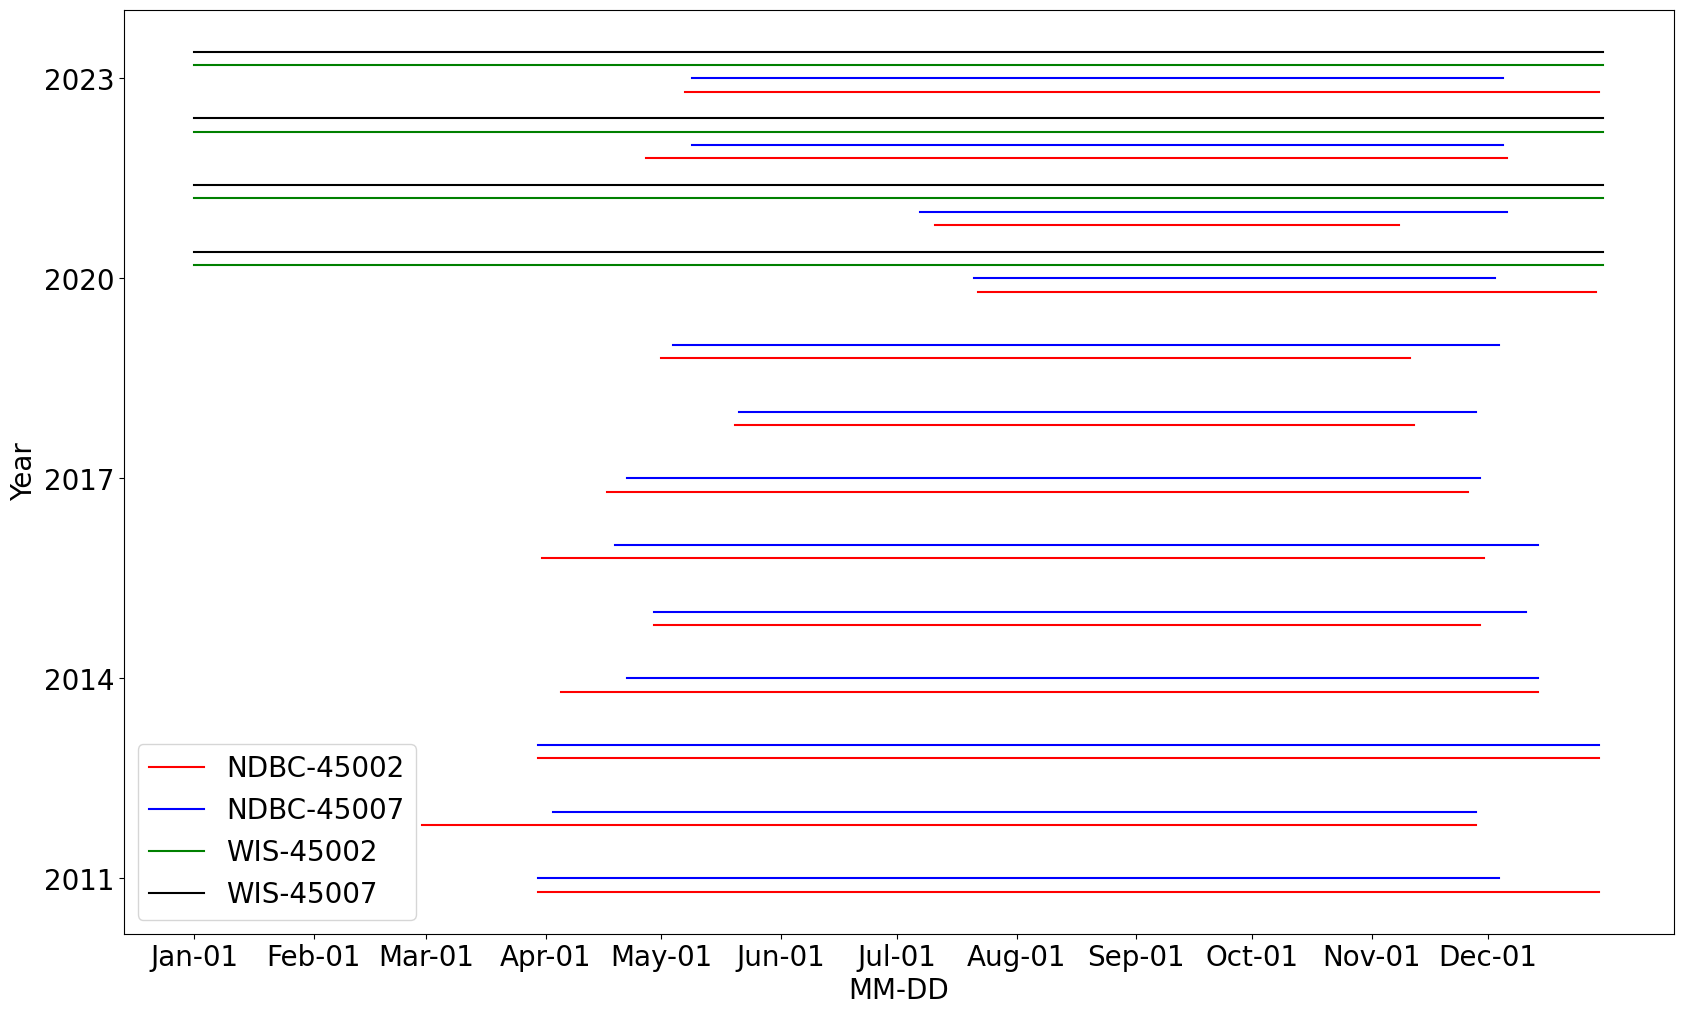
\includegraphics[width=0.8\textwidth]{chapter4/resources/figure4-2.png}
  \caption{Data availability for wave spectral data in NDBC and WIS station 45002 and 45007.}
  \label{fig:fig4.2}
\end{figure}

The Wave Information Study (WIS) is a wave hindcasting project that employs
hydrodynamic models to simulate design wave data along the United States
coastline. In the Great Lakes, the numerical model employed is WAM, a
third-generation wave model that solves the energy balance equation, accounting
for the impacts of wind and ice dynamics \citep{jensen_lake_2012}. WIS hindcast
data provides hourly wave climate in the nearshore of Lake Michigan starting
from 1979 to current. The spectral energy wave data provided by WIS includes 72
directional bands and 28 frequency bins, with frequency intervals based on ratio
0.0611 Hz. The wave climate data (\eg significant wave height, peak period) were
derived from the directional wave spectral data, with wind sea and swell
components partitioned using the method of WAM model
\citep{komen_dynamics_1994}. Here is the rule of Komen's WAM model:

\begin{equation}
    Check = f\frac{28\times u_*}{c(m)}(\cos(\theta_{wave}(k)-\theta_{wind}))
\label{eq:eq4.1}
\end{equation}

Where $f$ is the calibration factor,  $u_*$ is the friction wind speed, $c(m)$
is the phase speed defined at each frequency band (computed from the dispersion
relationship), $\theta_{wave}(k)$ is the wave angle defined at each directional
band, $\theta_{wind}$ is the wind direction, Check  is the criterion for the
partition with a value greater than 1 are classified as windsea waves. In
addition to the 490 coastal WIS station that provides hourly spectral wave data
since 1979 in Lake Michigan, WIS operates two stations in the central region of
Lake Michigan.  These central stations are used to validate the model against
wave measurement data obtained from the National Data Buoy Center (NDBC). These
two WIS stations can be accessed through the Coastal Hydraulic Laboratory (CHL)
THREDDS Data Server
(\url{https://chldata.erdc.dren.mil/thredds/catalog/catalog.html}). However,
data availability is limited to only four years from 2020 (see Figure
\ref{fig:fig4.2}). Due to the limited availability of data in the central Great
Lakes, in this study, the WIS spectral data in the 45002 and 45007 will only be
used to validate the partitioning results, as it provides partitioned swell and
wind-sea wave climates.

Nation Data Buoy Center (NDBC) provides detailed spectral wave data obtained
from meteorology buoys placed by NOAA. In Lake Michigan, NOAA placed two
MetOcean buoys in the center of lake (45002, 45007) and sixteen coastal gauges
(GLOS). NDBC buoy 45002 is a 2.1-meter ionometer foam buoy located in northern
Chippewa Basin at a depth of 181.4 meters, while buoy 45007 is a 2.3-meter foam
discus buoy located in southern Chippewa basin at a depth of 159.1 meters. Two
buoys provided documented meteorological data including wave speed, wave
direction, wind speed and wind direction since 1979 for 45002 and 1981 for
45007, respectively. The two buoys also provided spectral wave data derived from
heave acceleration and the vertical displacement of the buoy hull, measured
using onboard accelerometers or inclinometers. These spectral records have been
documented during ice-free seasons since 2011 for both 45002 and 45007 (see
Figure \ref{fig:fig4.2}). The spectral data provided by the hull encompasses
spectral wave density, mean wave direction, principal wave direction, and two
directional Fourier coefficients. The NDBC buoys did not measure a directional
wave spectrum, instead, construct by the Fourier analysis
\citep{longuet-higgins_observations_1961}. Here is the procedure of constructing
directional spectra.

\begin{equation}
    S(f,\theta) = c(f)D(f,\theta)
\label{eq:eq4.2}
\end{equation}

\begin{equation}
    D(f,\theta)=\frac{0.5+r_1\cos(\theta-\theta_1)+r_2\cos(\theta-\theta_2)}{\pi}
\label{eq:eq4.3}
\end{equation}

Where $c(f)$ is the energy density spectrum in the frequency band $f$, $r_1$ and
$r_1$ are the directional Fourier coefficients measured by the hull, $\theta_1$
and $\theta_2$  are the mean and principal wave direction measured by the hull,
$\theta$ is the directional band which is chosen as 5 degree. which poses
challenges when applying logarithmic transformations in the analysis. To
eliminate this negative value, \citet{earle_use_1999} provided an approach by
weighing the coefficients in the equation \ref{eq:eq4.3} as following.

\begin{equation}
    D(f,\theta)=\frac{0.5+\frac{2}{3}r_1\cos(\theta-\theta_1)+\frac{1}{6}r_2\cos(\theta-\theta_2)}{\pi}
\label{eq:eq4.4}
\end{equation}

This approach ensures that most wave climate statistics, including significant
wave height, peak wave period, and peak wave direction, remain consistent with
the original spectrum. However, it may also introduce bias in the representation
of directional wave spreading. In this study, the wave directional spectrum is
divided into 72 directional bands, each at 5-degree intervals starting from 0
degrees. The wave frequency spectrum is partitioned into 38 frequency bands,
determined by a ratio of 0.11 and starting at 0.03 Hz.

\subsection{Wave spectral partitions}
\label{Wave spectral partitions}

\begin{figure}[htbp]
  \centering
  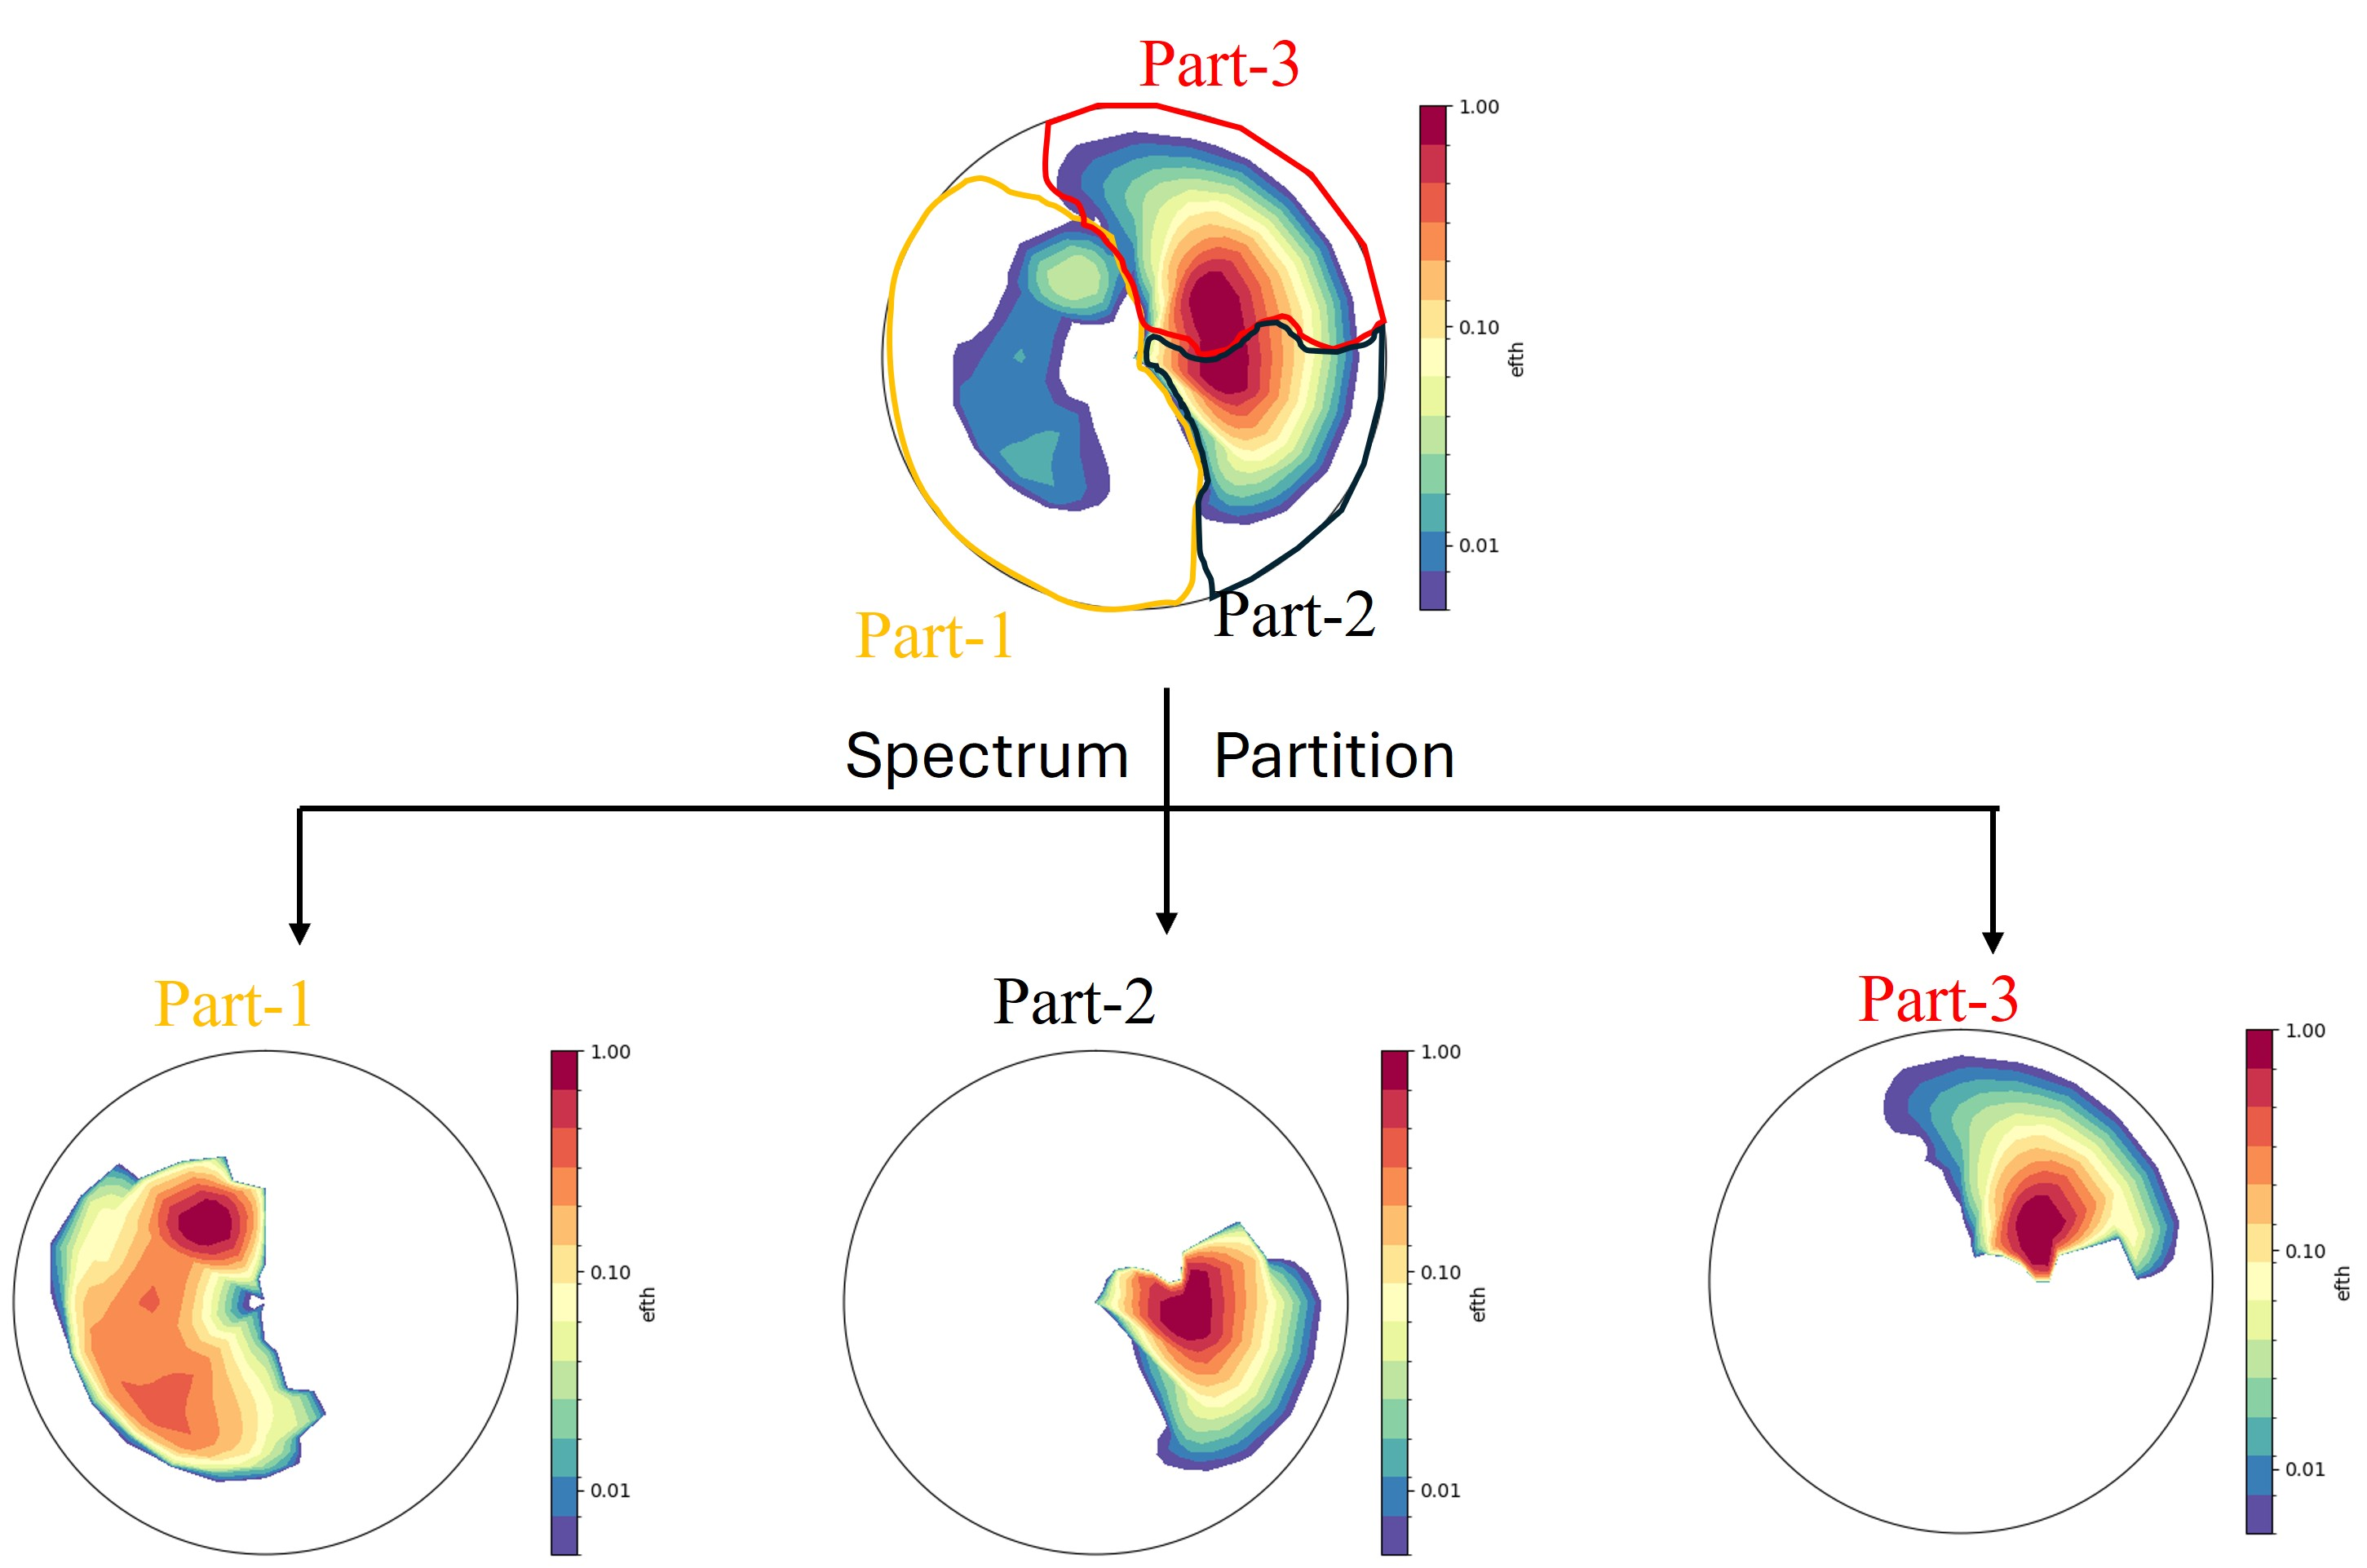
\includegraphics[width=0.8\textwidth]{chapter4/resources/figure4-3.jpg}
  \caption{Schematic of wave spectrum partition}
  \label{fig:fig4.3}
\end{figure}

Wave spectrum partitioning is a technique that decomposes a wave energy spectrum
into several sub-divisions, each of which corresponds to an individual wave
event \citep{portilla-yandun_wave_2015}. Figure \ref{fig:fig4.3} presents a
schematic of wave spectrum partitioning, in which a bulk wave spectrum is
divided into three components, each representing an individual wave event
originating from a distinct direction. The wave partition algorithm follows the
framework of previous work of watershed method \citep{hanson_automated_2001} and
smoothing method \citep{portilla_spectral_2009,portilla-yandun_wave_2015}. The
first step in the partitioning process involves preprocessing the constructed
spectra by smoothing the directional spectra using a 3*3 convolution kernel.
This means that each entry in the directional spectrum is averaged with its
neighboring entries to reduce noise and ensure smoother data. Second, from each
frequency–direction spectral bin, the steepest ascending path of variance
density is traced until a local peak is identified and all the points climbing
to the same local peak are grouped, and together they constitute a partition.
The third step involves merging partitions with low energy until the total
number of partitions is equal to or less than a predefined threshold. This study
utilized an open-source Python library, wavespectra, which provides
implementations of numerous partition algorithms (GitHub url:
\url{https://github.com/wavespectra/wavespectra}).  The library accepts several
arguments, including the directional wave spectrum represented as a $38\times72$
matrix for the frequency-directional domain, wind speed, wind direction, age
factor, and maximum number of partitions. The age factor serves as a criterion
to distinguish between swell and wind-sea, as described in the following
statement.


\begin{equation}
    \beta\frac{U_z}{c_p}\cos(\theta-\varphi) > 1
\label{eq:eq4.5}
\end{equation}

Where $\beta$ is age factor, $U_z$ is the wind speed at elevation $z$, $c_p$ is
the phrase speed determined by dispersion relationship, $theta$ is wave
direction, and $\varphi$ is wind direction. This approach follows Komen’s WAM
configuration, which is also utilized in the WIS framework (as outlined in
Equation \ref{eq:eq4.1}). In this study, the number of partitions was set to
three, resulting in one wind-sea component and two swell components. Various age
factors (1.2, 1.3, 1.5, and 1.7) were tested by comparing the generated
partitioning results with existing partitions from WIS and NDBC from 2020 to
2023. Then, an optimal age factor then was chosen to generate long-term wave
system partition in 45002 to 45007 from 2011 to 2023. 

\subsection{Directional spectral wave climate analysis}
\label{Directional spectral wave climate analysis}

Wave system partitioning provides one wind-sea partition spectrum and two swell
partitions spectrum at each hour from 2011 to 2023. The wave spectra were then
used for calculating the integrated wave climate including significant wave
height $H_s$, peak wave height $T_p$, and peak wave direction $\theta_p$ for
wind-sea and swell.  

\begin{equation}
    H_s=4\times \sqrt{\int \int S(f,\theta)dfd\theta}
\label{eq:eq4.6}
\end{equation}

\begin{equation}
    T_p=\frac{1}{\arg\max_f \int S(f,\theta)d\theta}
\label{eq:eq4.7}
\end{equation}

\begin{equation}
    \theta_p=\arg\max_f \int S(f,\theta)df
\label{eq:eq4.8}
\end{equation}


Moreover, the wave spectrum provides spatial information about the wave systems
within the frequency-direction domain. To capture this information, the peak
position of each wave system partition was extracted to characterize the wave
system’s properties within the spectrum \citep{portilla-yandun_wave_2015}. The
next step involves collecting all peak positions of the wave system partitions
across the entire time series from 2011 onward and counting the frequency of
occurrences of these peaks within the frequency-direction domain. This
distribution of occurrences within the frequency-direction domain was
subsequently used to analyze various aspects, including wave directionality,
modality, inter-annual trends, and intra-annual trends. Meanwhile, at each timestamps,
wave system will be classified into three different conditions: wind-sea dominant,
swells dominant and mixed conditions, which defined by $K$ in the following equations:

\begin{equation}
K = \frac{m_{0ws}}{m_{0tot}}
\label{eq:eq4.9}
\end{equation}

where $m_{0ws}$ is the zeroth order of moment of wind-sea partitions, and
$m_{0tot}$ is the zeroth order of moment of total wave energy spectrum.
Thresholds (0.25, 0.75) of wave systems conditions were selected based on
\citet{mazzaretto2024worldwide}'s metric and presented as following,

\begin{equation}
\begin{cases}
\text{wind-sea domiant} & \text{if } K \geq 0.75 \\
\text{sea domiant} & \text{if } K \leq 0.25 \\
\text{mixed condition} & \text{if } 0.25 < K < 0.75
\end{cases}
\label{eq:eq4.10}
\end{equation}

\section{Results}
\label{c4_results}

\subsection{Wave spectrum constructing and partitions}
\label{Wave spectrum constructing and partitions}

\begin{figure}[htbp]
  \centering
  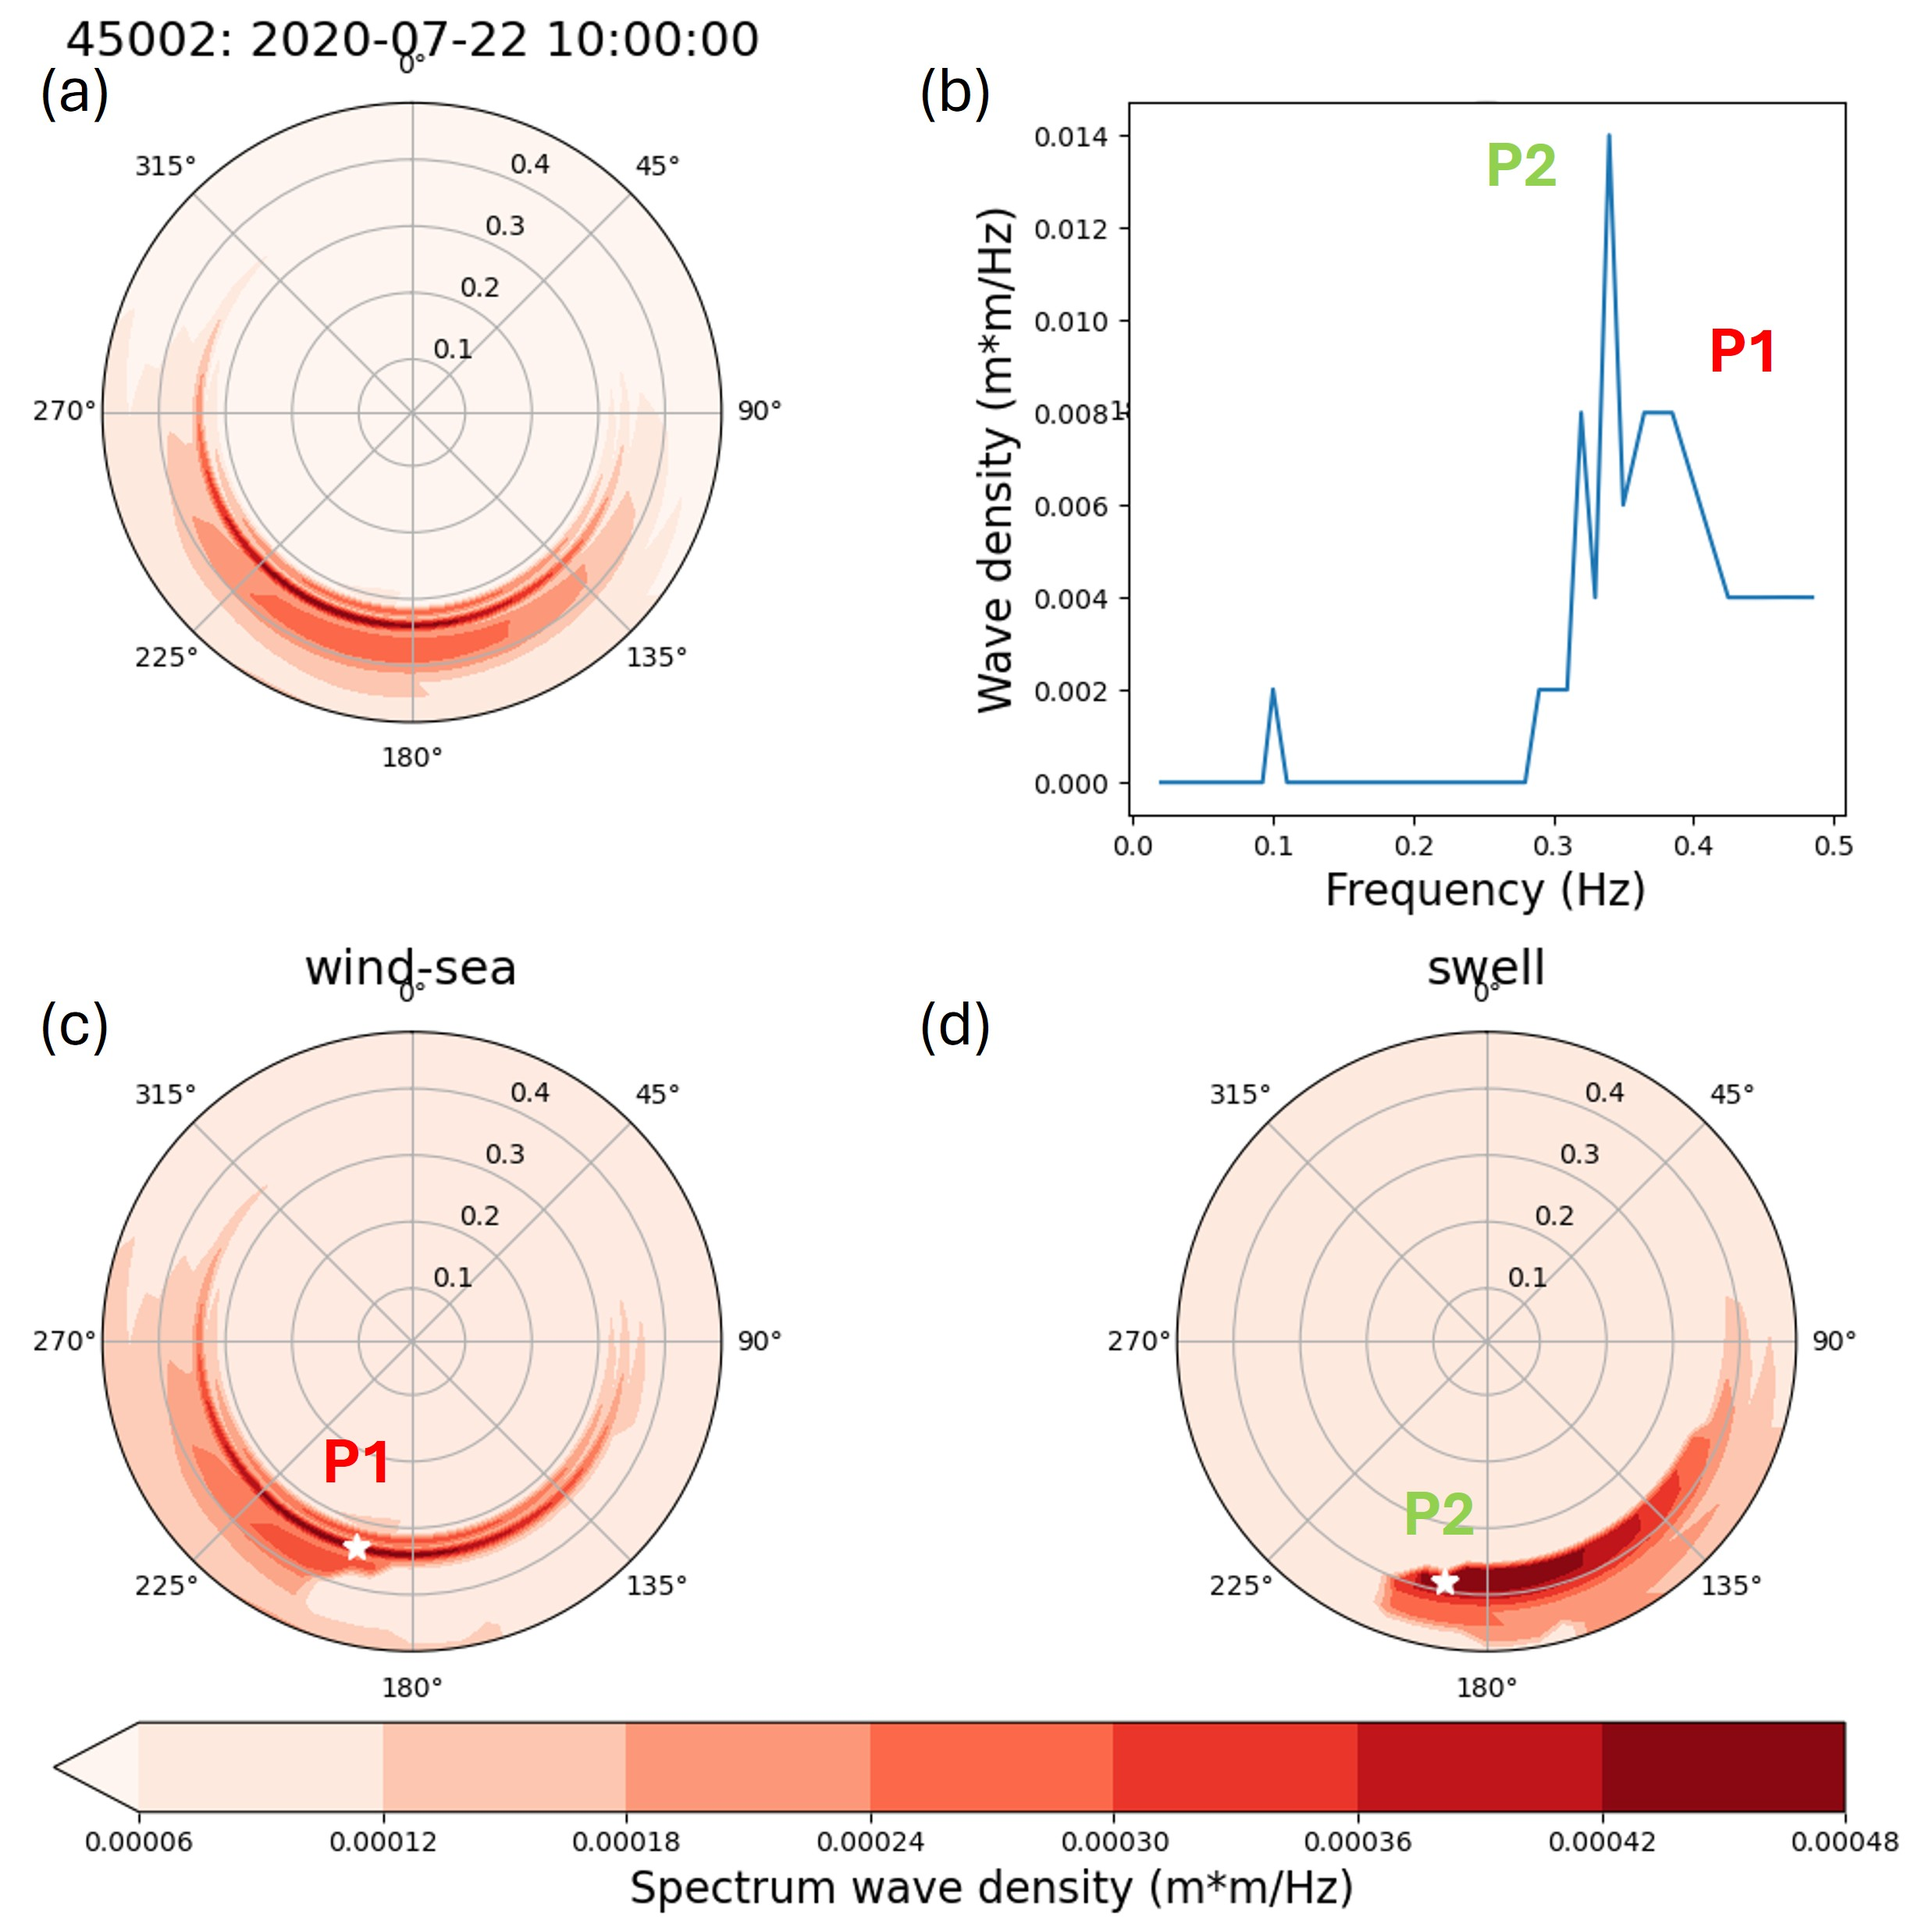
\includegraphics[width=0.7\textwidth]{chapter4/resources/figure4-6.jpg}
  \caption{The results of wave constructing and partitions are illustrated with
  an example from 45002 on 2020-07-22, 10 am including (a) construction of
  directional wave spectrum (b) domain of wave frequency-density energy (c)
  partition of wind-sea (d) partition of swell}
  \label{fig:fig4.6}
\end{figure}

\begin{table}[htbp]
\centering
\caption{Summary of partition results in NDBC stations 45002 and 45007 (mean $\pm$ std)}
\label{tab:tab4.1}
\begin{tabular}{|l|c|c|c|c|}
\hline
\multicolumn{5}{|c|}{\textbf{NDBC 45002}} \\ \hline
\textbf{Partitions} & \textbf{Count} & $H_s$ (m) & $t_p$ (s) & $\theta_p$ (deg) \\ \hline
Wind-sea & 37,023 & 0.66 $\pm$ 0.53 & 3.82 $\pm$ 1.11 & 217 $\pm$ 37 \\ \hline
Swell    & 46,923 & 0.41 $\pm$ 0.43 & 4.59 $\pm$ 2.42 & 189 $\pm$ 36 \\ \hline
Total    & 56,087 & 0.66 $\pm$ 0.57 & 4.31 $\pm$ 1.51 & 201 $\pm$ 36 \\ \hline
\multicolumn{5}{c}{} \\[-6pt] \hline
\multicolumn{5}{|c|}{\textbf{NDBC 45007}} \\ \hline
\textbf{Partitions} & \textbf{Count} & $H_s$ (m) & $t_p$ (s) & $\theta_p$ (deg) \\ \hline
Wind-sea & 35,925 & 0.67 $\pm$ 0.58 & 3.78 $\pm$ 1.14 & 189 $\pm$ 36 \\ \hline
Swell    & 44,774 & 0.41 $\pm$ 0.42 & 4.64 $\pm$ 2.22 & 14 $\pm$ 34  \\ \hline
Total    & 55,245 & 0.65 $\pm$ 0.60 & 4.23 $\pm$ 1.33 & 101 $\pm$ 33 \\ \hline
\end{tabular}
\end{table}


The wave spectrum was constructed and partitioned at every hour in 45002 and
45007 from 2011 to 2023. Figure \ref{fig:fig4.6} shows the result of wave
spectrum construction and wave system partition in station 45002 on 2020-07-22,
10 am. The two partitions: wind-sea (Figure \ref{fig:fig4.6} c) and swell
(Figure \ref{fig:fig4.6} d) are arranged in descending order of frequency, as
illustrated in the wave frequency-energy domain presented in Figure
\ref{fig:fig4.6} b. This arrangement aligns with the physical characteristics of
wind-sea and swell waves: wind-sea corresponds to the high-frequency portion of
the wave spectrum, while swell is associated with the low-frequency portion of
the spectrum. The peak positions of partitions (\eg $P_1$, $P_2$ in Figures
\ref{fig:fig4.6}c, d) were also extracted for further analysis of wave event
occurrences, which will be discussed in the next section. 

Meanwhile, key wave parameters such as the significant wave height $H_s$, peak
wave angle $\theta_p$ and peak frequency $f_p$ were extracted from each
partition and aggregated to generate long-term statistics covering the period
from 1996 to 2023 (Table \ref{tab:tab4.1}) after excluding null and zero-value
partitions during icy seasons. At Station 45002, about 56k partitions were
identified, including roughly 37k wind-sea events and 47k swell events.  At
Station 45007, a comparable number of partitions (about 55k) were recorded, with
approximately 36k wind-sea and 45k swell events, indicating a similar balance
between the two wave systems. The mean significant wave height ($H_s$) is nearly
identical at the two sites (0.66 $\pm$ 0.57 m at 45002 and 0.65 $\pm$ 0.60 m at
45007). Peak periods ($t_p$) also remain close, with slightly longer waves
observed at Station 45002 (4.31 $\pm$ 1.51 s) compared to Station 45007 (4.23
$\pm$ 1.33 s). In terms of wave direction, however, the stations diverge. At
45002, wind-sea events ($H_s = 0.66 \pm 0.53$ m, $t_p = 3.82 \pm 1.11$ s)
predominantly travel from the west-southwest (217$^\circ \pm$ 37$^\circ$), while
swell events ($H_s = 0.41 \pm 0.43$ m, $t_p = 4.59 \pm 2.42$ s) are oriented
southward (189$^\circ \pm$ 36$^\circ$). The combined sea state is dominated by
waves propagating eastward (201$^\circ \pm$ 36$^\circ$). In contrast, at Station
45007, wind-sea conditions are similar in energy ($H_s = 0.67 \pm 0.58$ m, $t_p
= 3.78 \pm 1.14$ s) with a predominant direction of 189$^\circ \pm$ 36$^\circ$, 
whereas swell events ($H_s = 0.41 \pm$ 0.42 m, $t_p = 4.64 \pm$ 2.22 s) are
mainly north-northeasterly (14$^\circ \pm$ 34$^\circ$). Consequently, the
overall sea state at 45007 exhibits a dominant northeastward orientation 
(101$^\circ \pm$ 33$^\circ$), in contrast to the eastward dominance at 45002.

\subsection{Validation of wave spectrum partitioning}
\label{Validation of wave spectrum partitioning}

\begin{figure}[htbp]
  \centering
  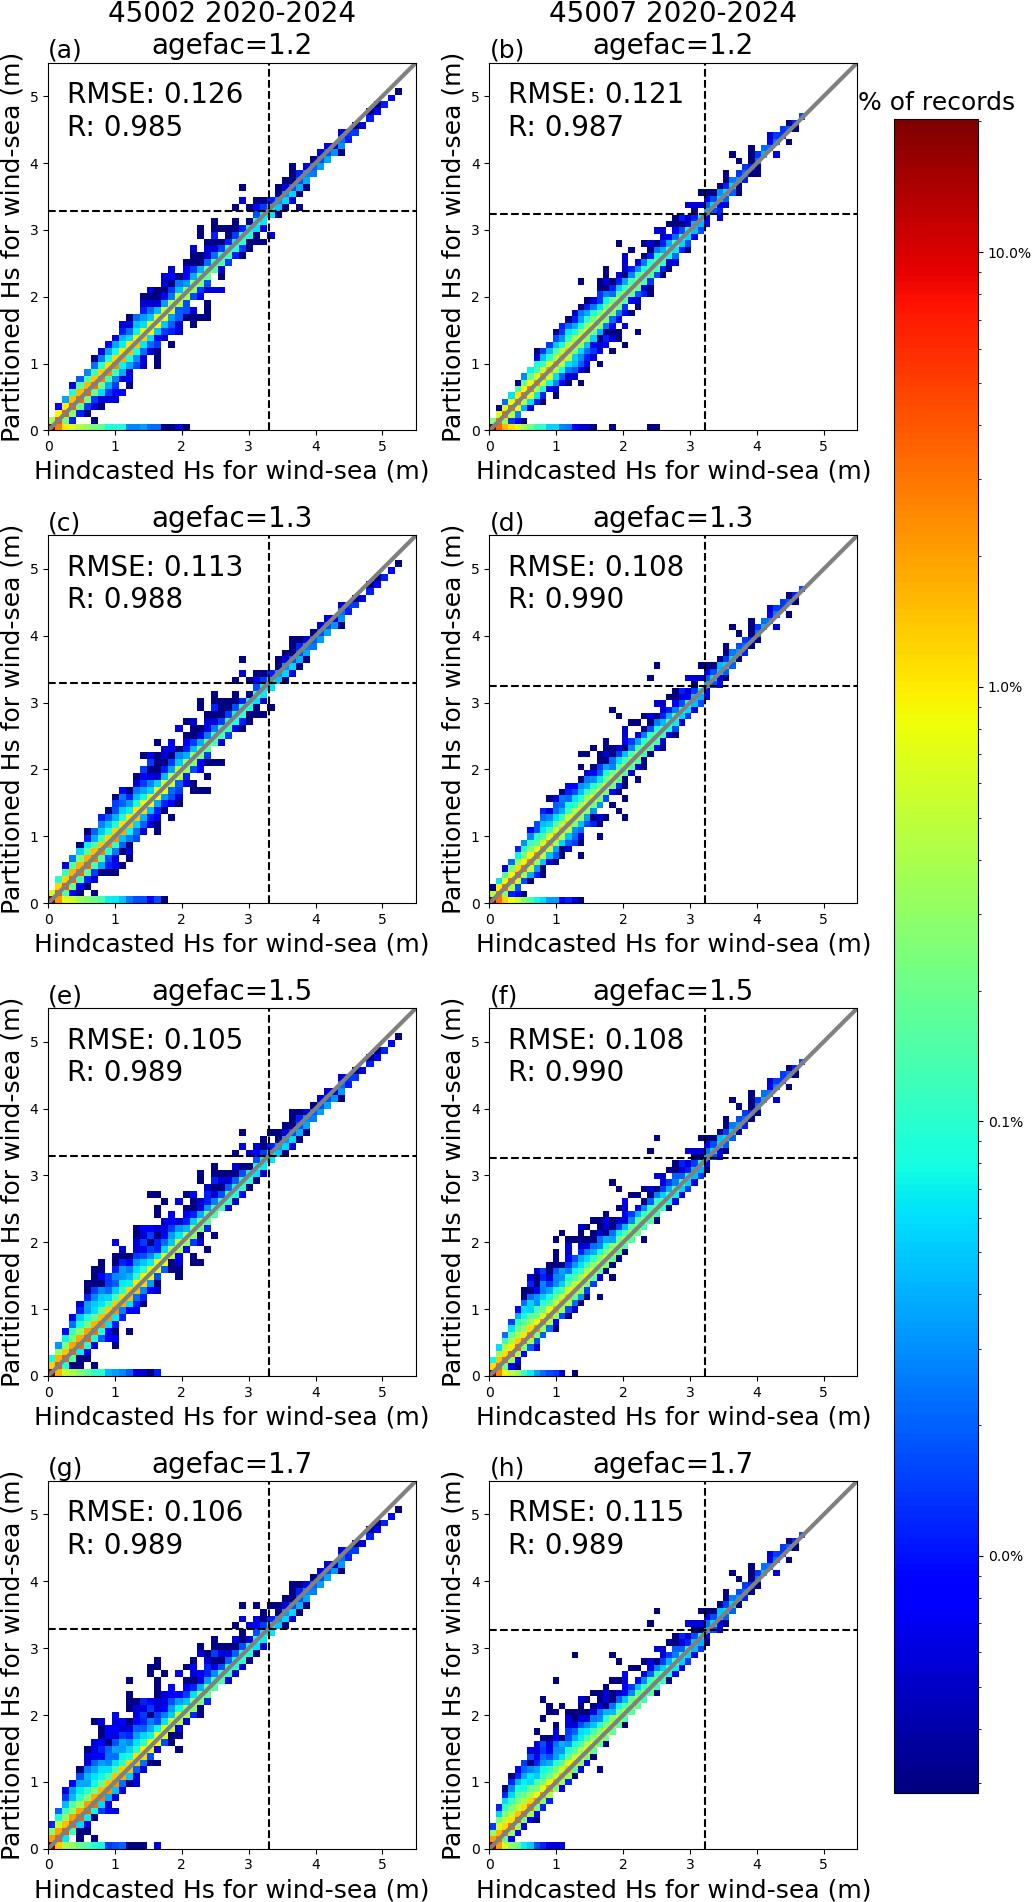
\includegraphics[width=0.7\textwidth]{chapter4/resources/figure4-4.jpg}
  \caption{scatter plots of hindcast wind-sea wave height modeled by WIS
  (x-axis) verse partitioned wind-sea wave height from our study (y-axis) in WIS
  45002 (left column) and 45007 (right column) with RMSE and R value. The
  scatter plot’s grid size is 0.1*0.1 meter.}
  \label{fig:fig4.4}
\end{figure}

Figure \ref{fig:fig4.4} shows scatter plots comparing wind-sea significant wave
heights (Hs) from this study’s partitioning method (x-axis) with those from WIS
partitions (y-axis). Only wind-sea results are presented, as WIS does not
provide sub-partitions within the swell domain. Two WIS stations—45002 (left
column) and 45007 (right column)—were analyzed for hourly wind-sea Hs from 2020
to 2024. Four wave age factors (1.2, 1.3, 1.5, and 1.7) were evaluated based on
Root Mean Square Error (RMSE) and correlation coefficient ($R$). Results
demonstrate strong agreement between this study’s partitioned wind-sea waves and
those of WIS, with low RMSE values (0.105–0.126) and high R values
(0.985–0.990). Among the tested age factors, 1.5 was selected as optimal,
yielding the lowest RMSE and highest R at both stations. Some scatter near the
x-axis suggests that the method occasionally underestimates wind-sea waves when
their magnitudes are very small.

\begin{figure}[htbp]
  \centering
  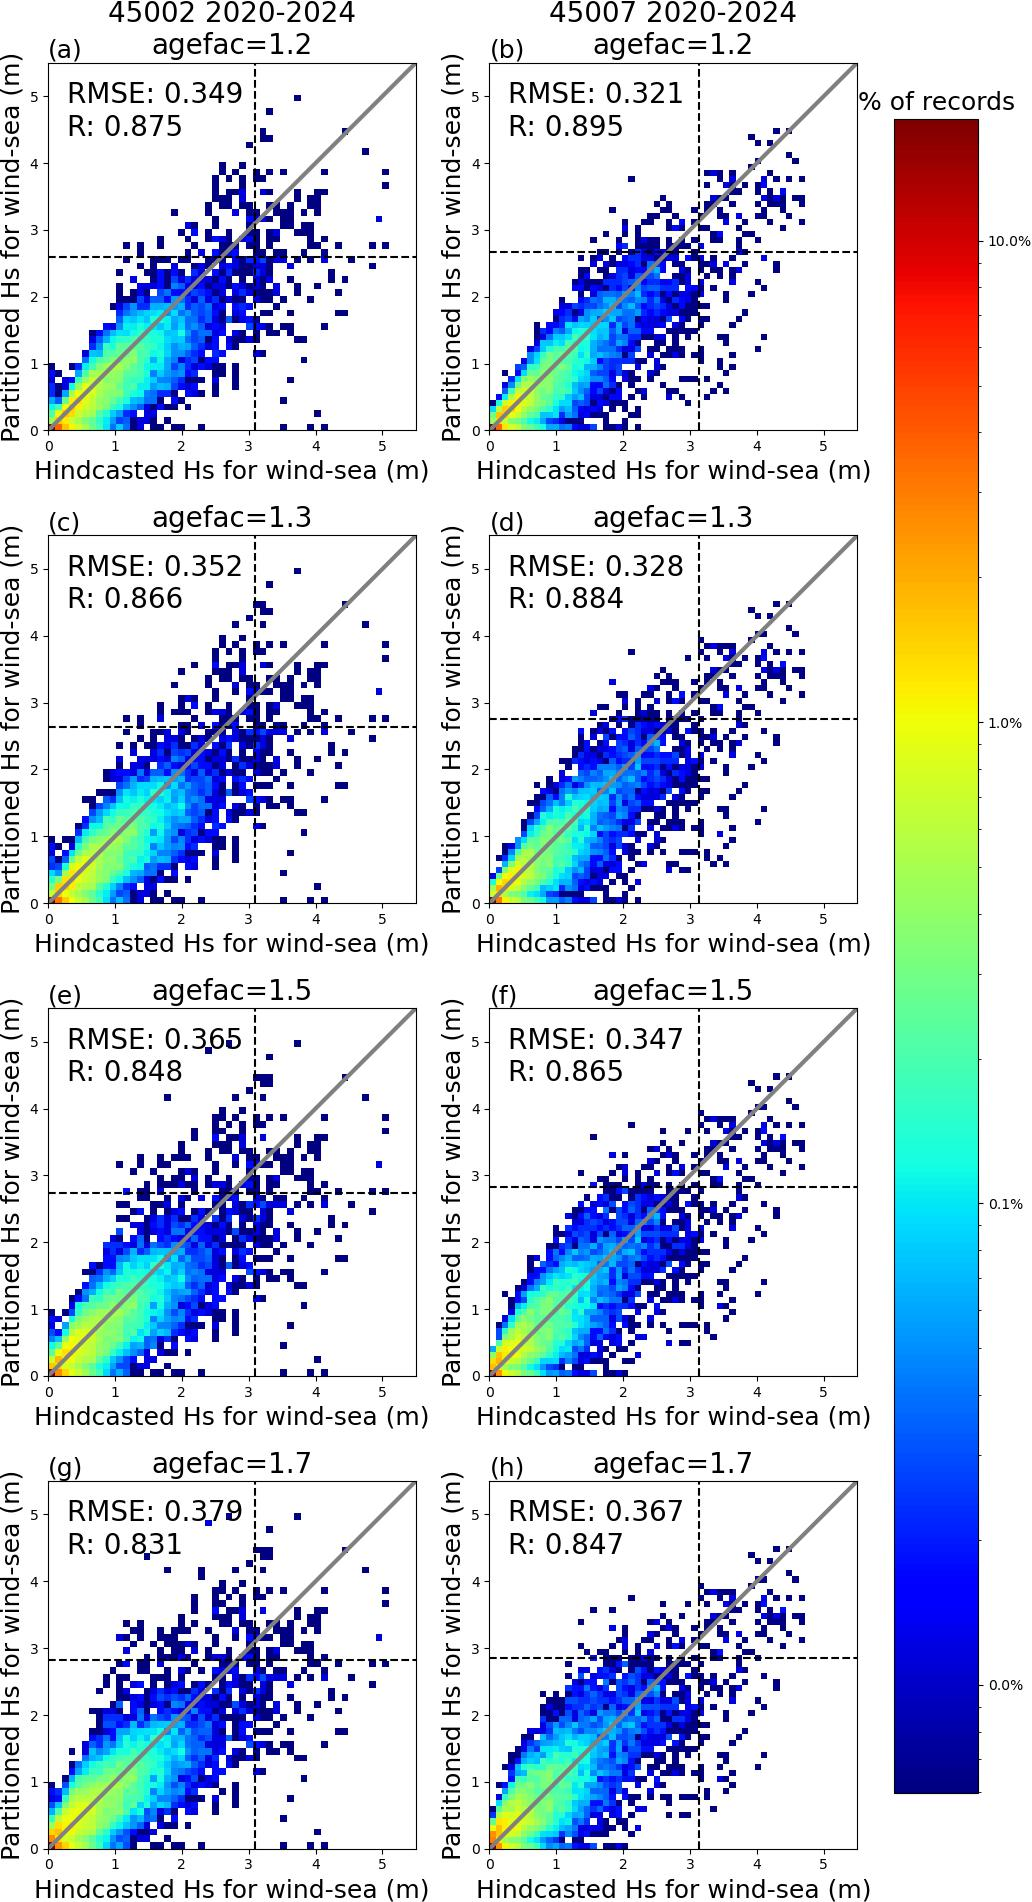
\includegraphics[width=0.7\textwidth]{chapter4/resources/figure4-5.jpg}
  \caption{scatter plots of hindcast wind-sea wave height modeled by NDBC
  (x-axis) verse partitioned wind-sea wave height from our study (y-axis) in
  NDBC 45002 (left column) and 45007 (right column) with RMSE and R value. The
  scatter plot’s grid size is 0.1*0.1 meter.}
  \label{fig:fig4.5}
\end{figure}

A similar analysis was conducted for NOAA-NDBC data at two stations, 45002 and
45007, as shown in Figure \ref{fig:fig4.5}. To maintain consistency with the WIS analysis,
the same duration from 2020 to 2024 was selected. The partitioning results for
NOAA-NDBC data are still promising, with relatively low RMSE values ranging from
0.321 to 0.379 and high correlation coefficients ($R$) ranging from 0.831 to
0.895. However, compared to the WIS results, the NOAA-NDBC partitions exhibit
greater bias, as indicated by the higher RMSE values compared to those in Figure
\ref{fig:fig4.4}. The reason for this discrepancy is that WIS is based on the WAM hindcast
model, which employs a wind-sea and swell partitioning approach similar to that
used in this study. In contrast, the NDBC results are derived from constructed
wave spectra, which introduces a relatively larger bias in the partitioning
process. Among the different wave age factors, the 1.2 were selected as it
presents the lowest RMSE and highest $R$ value than others.

Comparing the two partitions at hindcast wave (Figure \ref{fig:fig4.4}) verse gauges
(Figure \ref{fig:fig4.5}), several detailed patterns emerge. First, both stations show
consistent behavior: First, the density plots reveal that most records cluster
tightly along the 1:1 line, but at higher significant wave heights the
partitioned values tend to fall below the hindcast reference, indicating a
tendency toward underestimation in energetic sea states. Second, the color
scaling in the plots represents the percentage of records, which highlights the
dominance of small magnitudes waves ($Hs<1$) in the overall statistics and
underscores that the observed bias at higher $H_s$ stems from relatively fewer
but important extreme cases, especially for the gauges data in NDBC. Taken
together, these results suggest that while NOAA–NDBC partitions are broadly
reliable, their performance is more sensitive to wave-age tuning than the WIS
hindcast.

\subsection{Directional spectral wave climate in offshore regions}
\label{Directional spectral wave climate in offshore regions}

\begin{figure}[htbp]
  \centering
  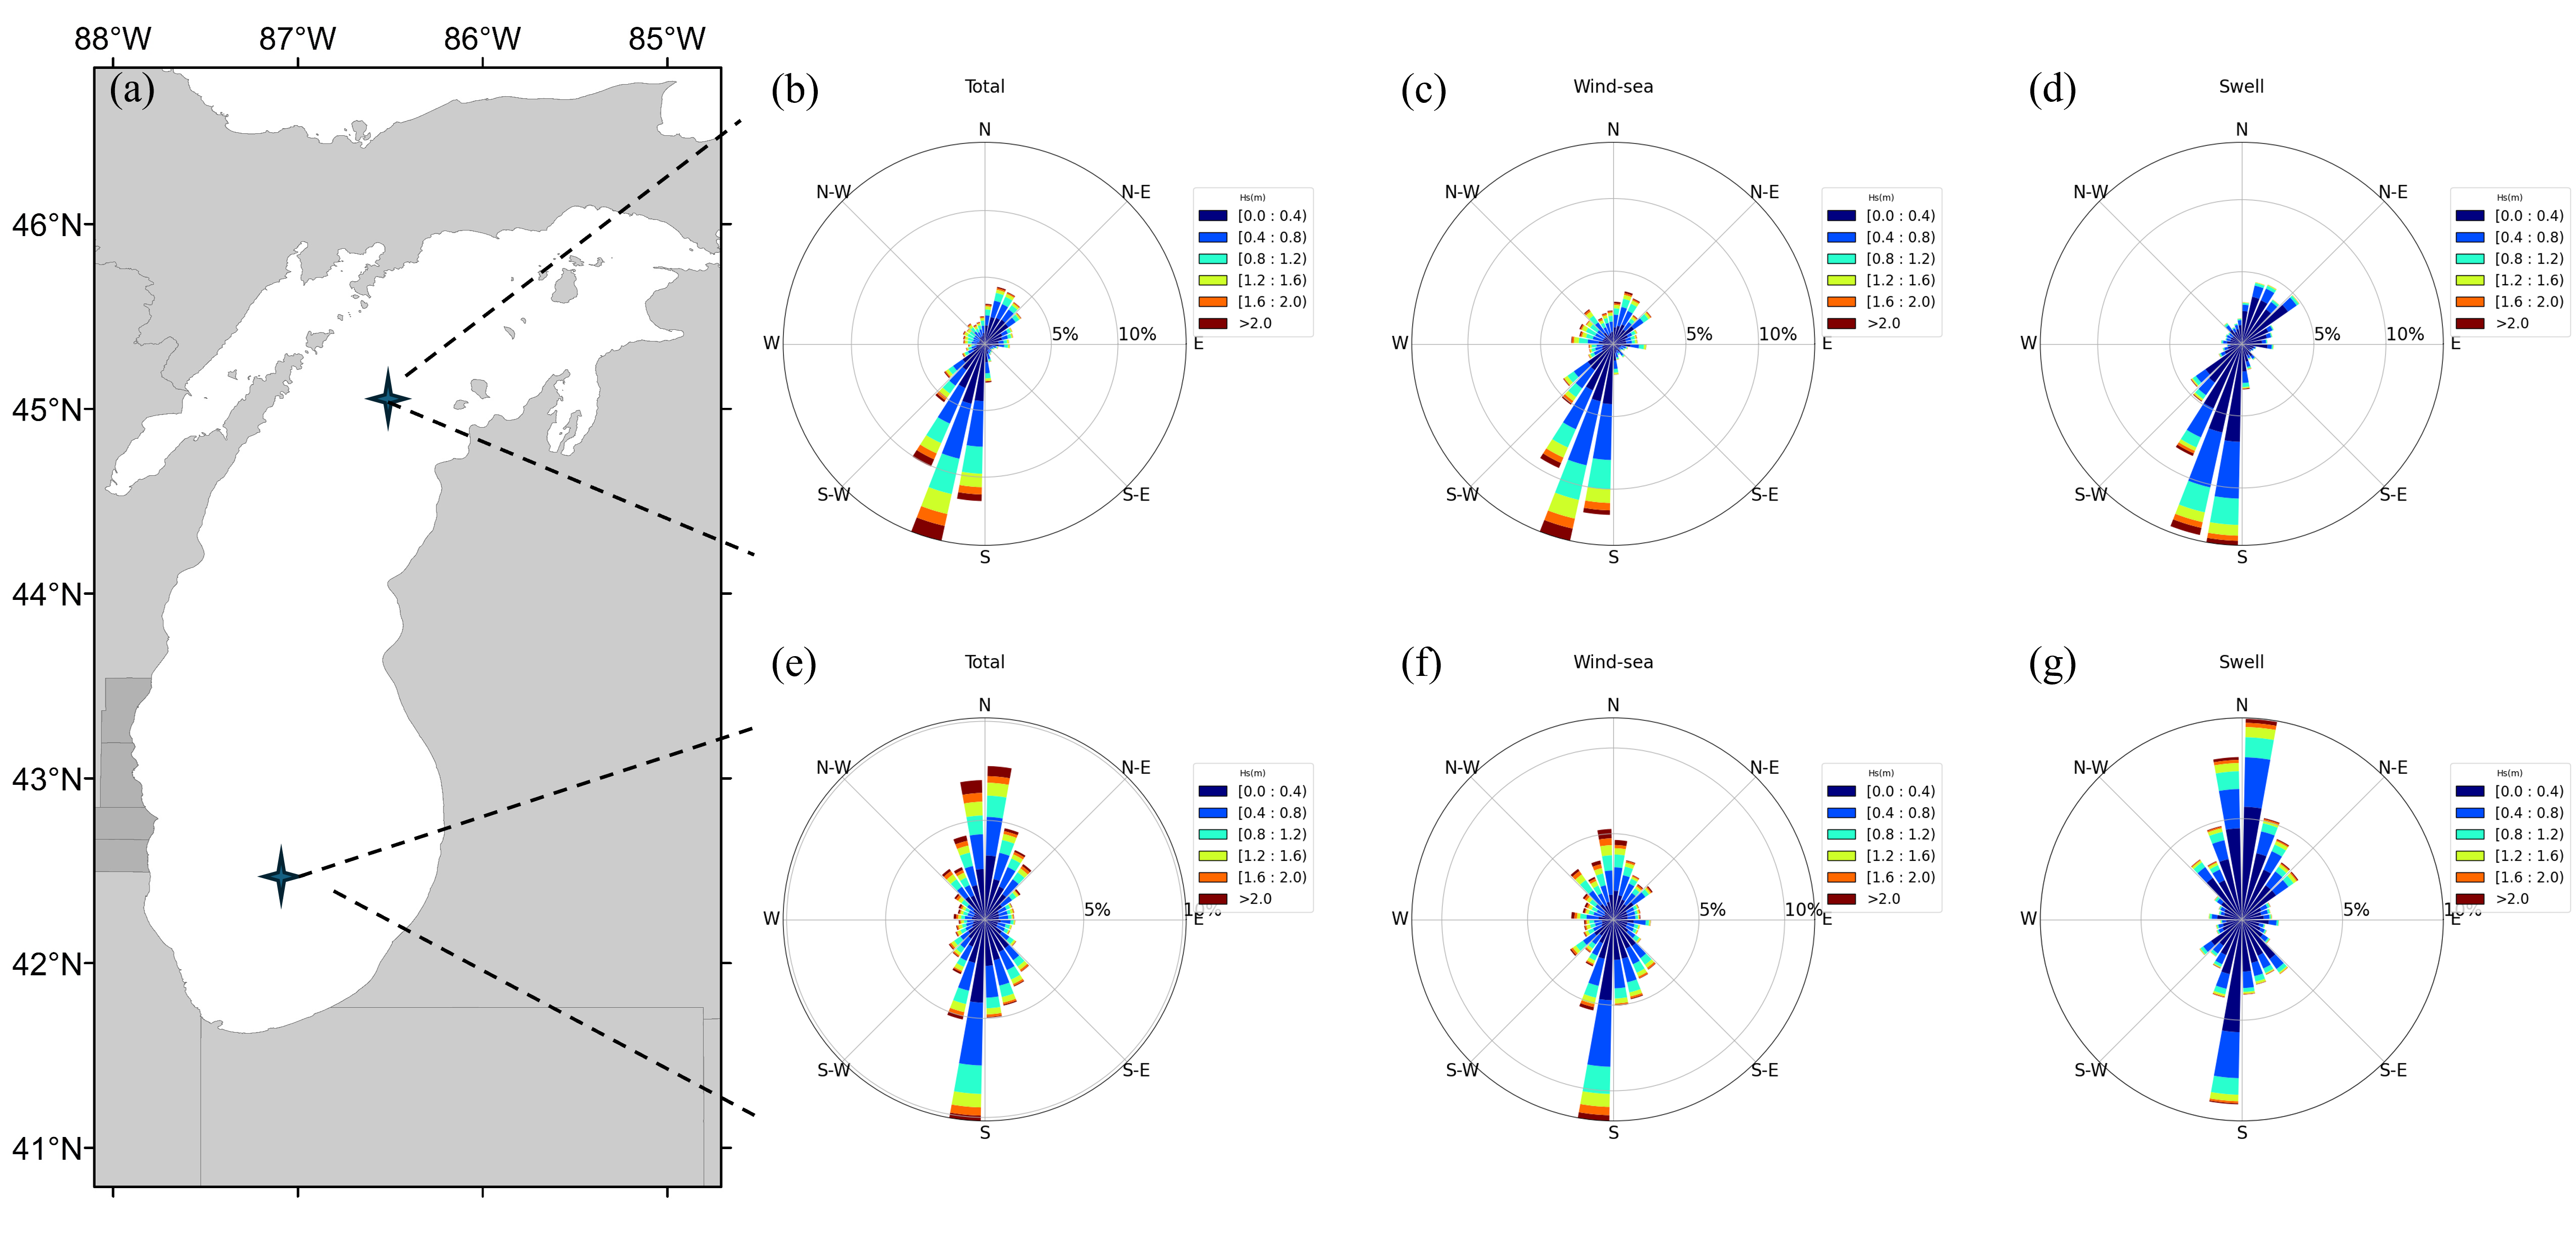
\includegraphics[width=1\textwidth]{chapter4/resources/ndbc_hs_rose.png}
  \caption{Significant wave height ($H_s$) wave roses in Lake Michigan. (a)
  locations of two NDBC buoys. (b) wave rose for total wave in 45002. (c) wave
  rose for wind-sea wave in 45002. (d) wave rose for swell wave in 45002. (e)
  wave rose for total wave in 45007. (f) wave rose for wind-sea wave in 45007.
  (g) wave rose for swell wave in 45007}
  \label{fig:ndbc_hs_rose}
\end{figure}

Wave roses of significant wave height ($H_s$) from 2011 to 2023 at two NDBC
buoys (45002 in the northern basin and 45007 in the southern basin; Figure
\ref{fig:ndbc_hs_rose}a) reveal strong spatial contrasts in the directional wave
climate of Lake Michigan. At the northern buoy (45002), the total wave field is
clearly unimodal, dominated by southerly waves (S–SSW; Figure
\ref{fig:ndbc_hs_rose}b). Most $H_s$ values fall between 0.4 and 1.2 m, but
storm conditions occasionally produce waves exceeding 2 m from the southwest,
reflecting the impact of intense southerly wind events over the limited fetch of
the northern basin. Partitioned spectra show that both wind-sea and swell
maintain similar southerly alignments (Figures \ref{fig:ndbc_hs_rose}c–d),
although they differ in extreme wave height. Wind-sea has more extreme wave
event ($H_s > 2$ m, the red bins in Figures \ref{fig:ndbc_hs_rose}c) from
northern direction, while swell is generally smaller in the northern waves. By
contrast, the southern buoy (45007) records a distinctly bidirectional regime.
The total wave field shows nearly symmetric contributions from both the north
and south (Figure \ref{fig:ndbc_hs_rose}e), with high-energy events above 2 m
occurring more frequently than at the northern site. Wind-sea energy is
distributed across both sectors (Figure \ref{fig:ndbc_hs_rose}f), highlighting
the influence of strong local winds acting along the long north–south fetch.
Swell waves also exhibit a pronounced bidirectional alignment (Figure
\ref{fig:ndbc_hs_rose}g), with contributions occasionally exceeding 2 m, which
underscores the southern basin’s exposure to long-distance wave propagation from
both directions.

\begin{figure}[htbp]
  \centering
  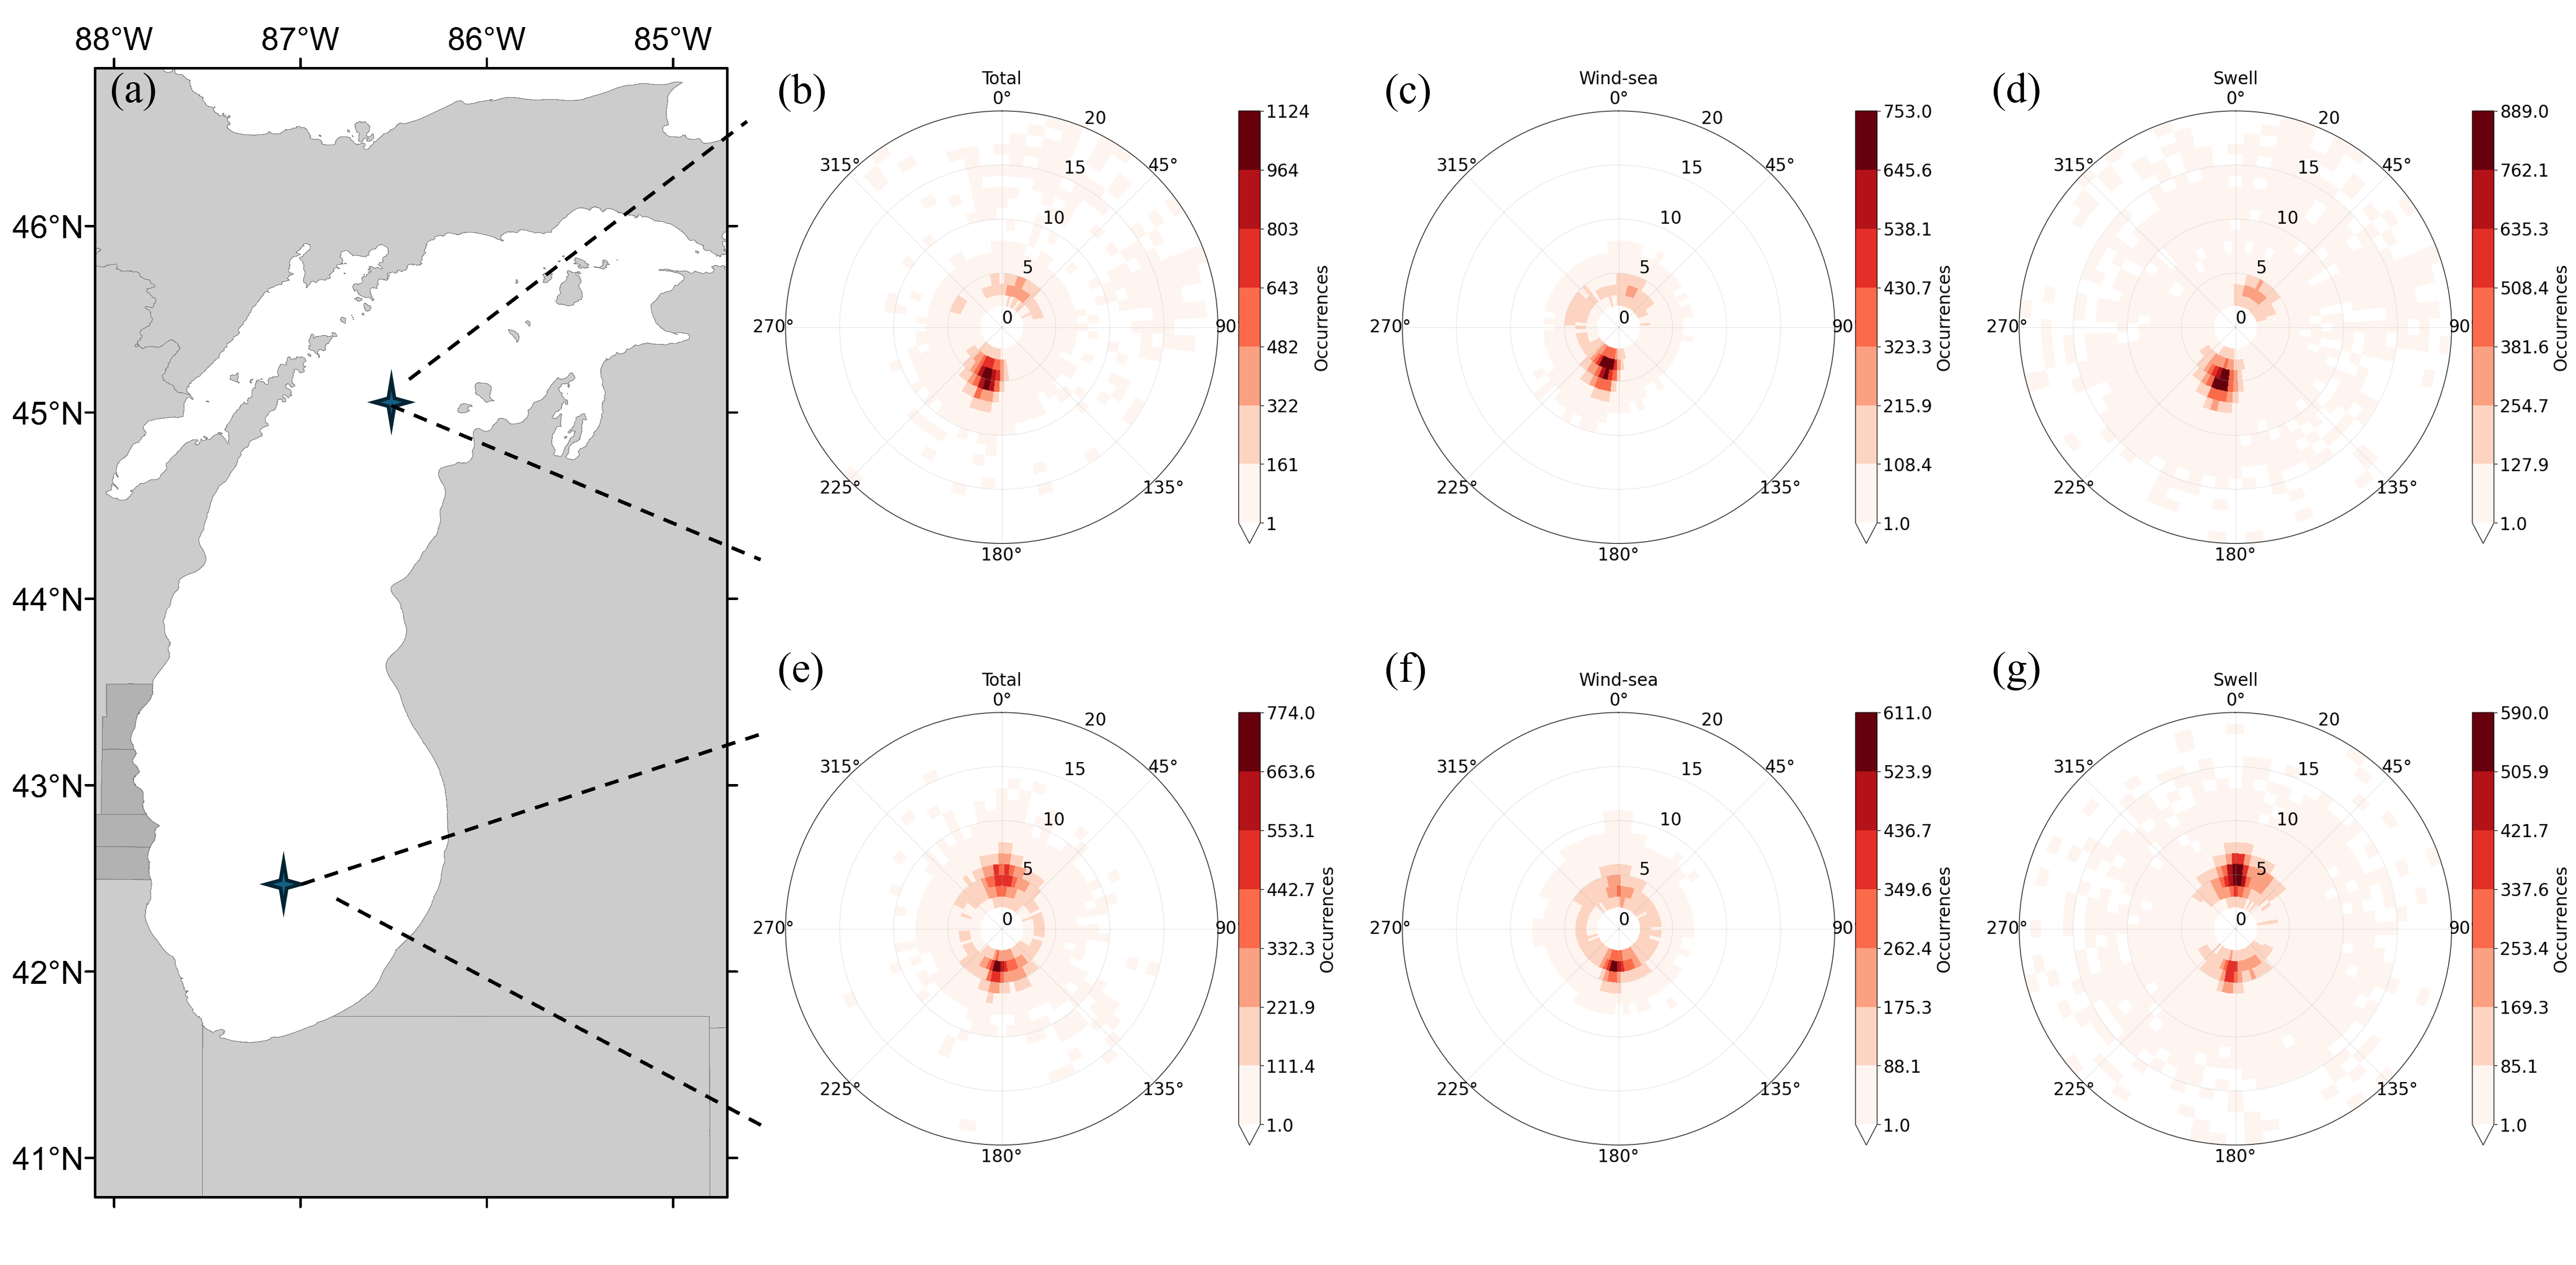
\includegraphics[width=1\textwidth]{chapter4/resources/ndbc_occ_rose.png}
  \caption{Wave peak period ($T_p$) wave occurrence map in Lake Michigan. (a)
  locations of two NDBC buoys. (b) wave rose for total wave in 45002. (c) wave
  rose for wind-sea wave in 45002. (d) wave rose for swell wave in 45002. (e)
  wave rose for total wave in 45007. (f) wave rose for wind-sea wave in 45007.
  (g) wave rose for swell wave in 45007}
  \label{fig:ndbc_occ_rose}
\end{figure}

The wave peak period ($T_p$) occurrence roses (Figure \ref{fig:ndbc_occ_rose}a)
provide further evidence of these spatial differences by illustrating the
spectral structure of the wave field. At the northern buoy (45002), wind-sea
events are dominated by short peak periods ($T_p < 5$ s), consistent with local
wave growth over limited fetches (Figures \ref{fig:ndbc_occ_rose}b–c). Swell
waves, in contrast, extend into longer periods ($T_p \approx 6$–8 s), and they
are equally frequent and generally eqivlent with wind-sea (Figure
\ref{fig:ndbc_occ_rose}d). Unlike wind-sea, swell also shows a broader
directional spread, with secondary contributions from the west and east (see the
pink regions in Figure \ref{fig:ndbc_occ_rose}d), suggesting occasional
cross-lake or refracted wave propagation. At the southern buoy (45007), the
bidirectional regime is even more evident in the period distributions. Wind-seas
remain short-period ($T_p < 6$ s) but occur almost equally from the north and
south (Figure \ref{fig:ndbc_occ_rose}f), consistent with frequent local
generation in both fetch directions. Swell waves at this site extend into
significantly longer periods ($T_p > 8$ s) and arrive from both directions
(Figure \ref{fig:ndbc_occ_rose}g), reflecting the ability of waves to propagate
across the full lake length. The higher frequency of long-period swell in the
south highlights its greater exposure to cross-basin forcing and long-fetch
dynamics.

Taken together, Figures \ref{fig:ndbc_hs_rose} and \ref{fig:ndbc_occ_rose}
confirm a pronounced north–south asymmetry in Lake Michigan’s spectral wave
climate. The northern basin is constrained by shorter fetches and dominated by
southerly, short-period wind-seas with limited swell influence, while the
southern basin is exposed to bidirectional forcing, producing a more energetic
regime that includes both frequent wind-sea extremes and long-period swell from
opposing directions. This spatial variability in wave height and period has
direct implications for sediment transport, shoreline erosion, and long-term
geomorphic change along different sectors of the lake’s coast.

\subsection{Inter- and Monthly- patterns of wave systems}
\label{Inter- and Monthly- patterns of wave systems}

\begin{figure}[htbp]
  \centering
  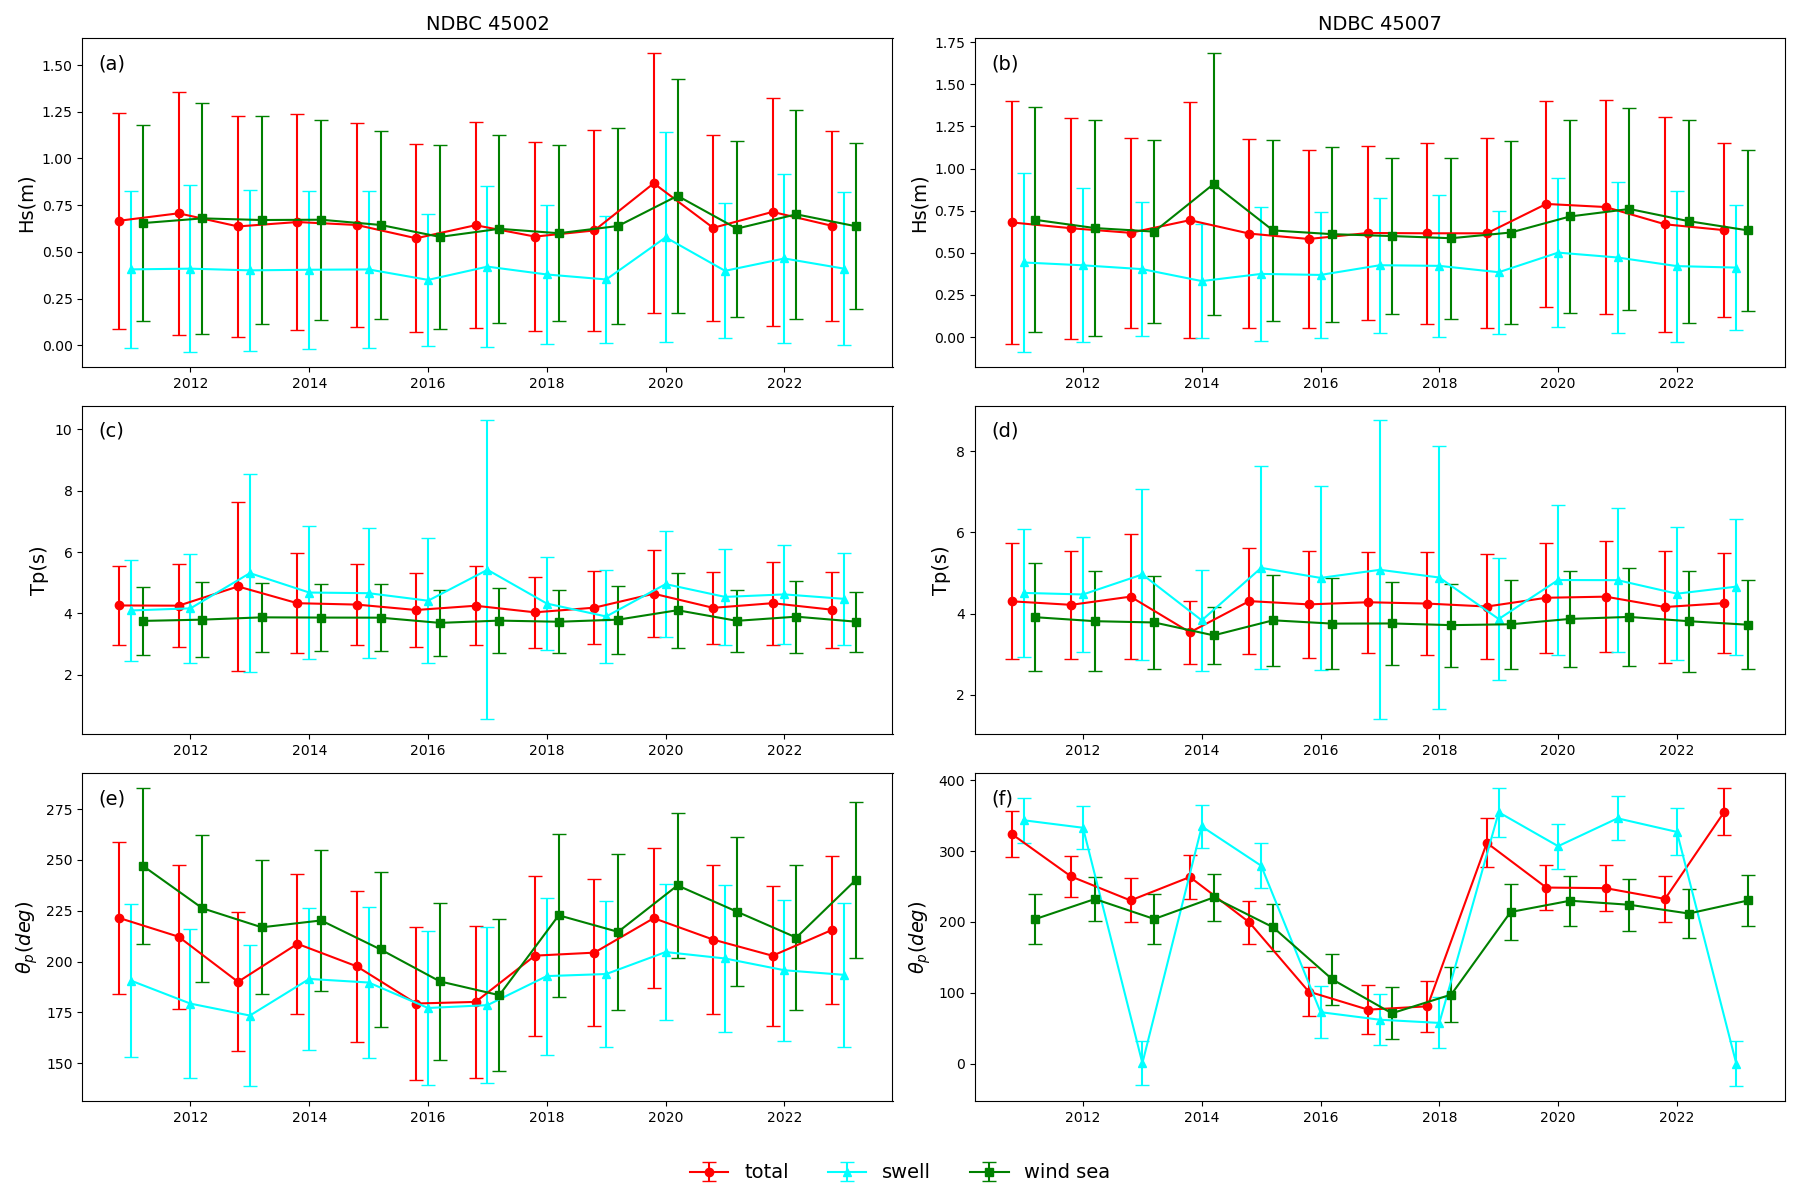
\includegraphics[width=1\textwidth]{chapter4/resources/ndbc_annual.png}
  \caption{Annual wave climates of NDBC stations 45002 and 45007, associated
  with each wave systems. (a-b) annual total, swell, and windseda $H_s$ in 45002
  and 45007, respectively, (c-d) annual total, swell, and windseda $T_p$ in
  45002 and 45007, respectively, (e-f) annual total, swell, and windseda
  $\theta_p$ in 45002 and 45007, respectively }
  \label{fig:ndbc_annual}
\end{figure}

Annual wave climates at NDBC buoys 45002 (northern basin) and 45007 (southern
basin) demonstrate marked spatial differences in significant wave height
($H_s$), peak period ($T_p$), and mean direction ($\theta_p$) across total,
swell, and wind-sea systems. At 45002, annual mean $H_s$ is relatively stable
(0.5–0.7 m) over 2011–2023, with limited interannual variability and extremes
primarily associated with wind-sea (Figure \ref{fig:ndbc_annual}a). Swell $H_s$
remains smaller and more consistent, reflecting the restricted fetch of the
northern basin. In contrast, 45007 exhibits consistently higher $H_s$ (0.6–0.9
m) with energetic years in 2012, 2016, and 2020, when annual averages of total
and wind-sea waves exceeded 1.0 m (Figure \ref{fig:ndbc_annual}b). Annual $T_p$
at 45002 is dominated by short periods (4–5 s for wind-sea, ~6 s for swell) with
little variability (Figure \ref{fig:ndbc_annual}c), whereas 45007 records longer
swell periods (6–8 s) with greater year-to-year variability, including
occasional extremes exceeding 8 s (Figure \ref{fig:ndbc_annual}d). Directional
patterns further emphasize the asymmetry: at 45002, all wave systems cluster
around southerly directions (~200–220°; Figure \ref{fig:ndbc_annual}e),
confirming its unimodal, fetch-limited character, while at 45007, annual mean
$\theta_p$ oscillates between north (~0–20°) and south (~180–200°), particularly
in the swell record (Figure \ref{fig:ndbc_annual}f). These results indicate that
the northern basin is dominated by short-period, southerly wind-sea with limited
variability, whereas the southern basin is more energetic, variable, and
bidirectional, sustaining both frequent wind-sea extremes and long-period swell.

\begin{figure}[htbp]
  \centering
  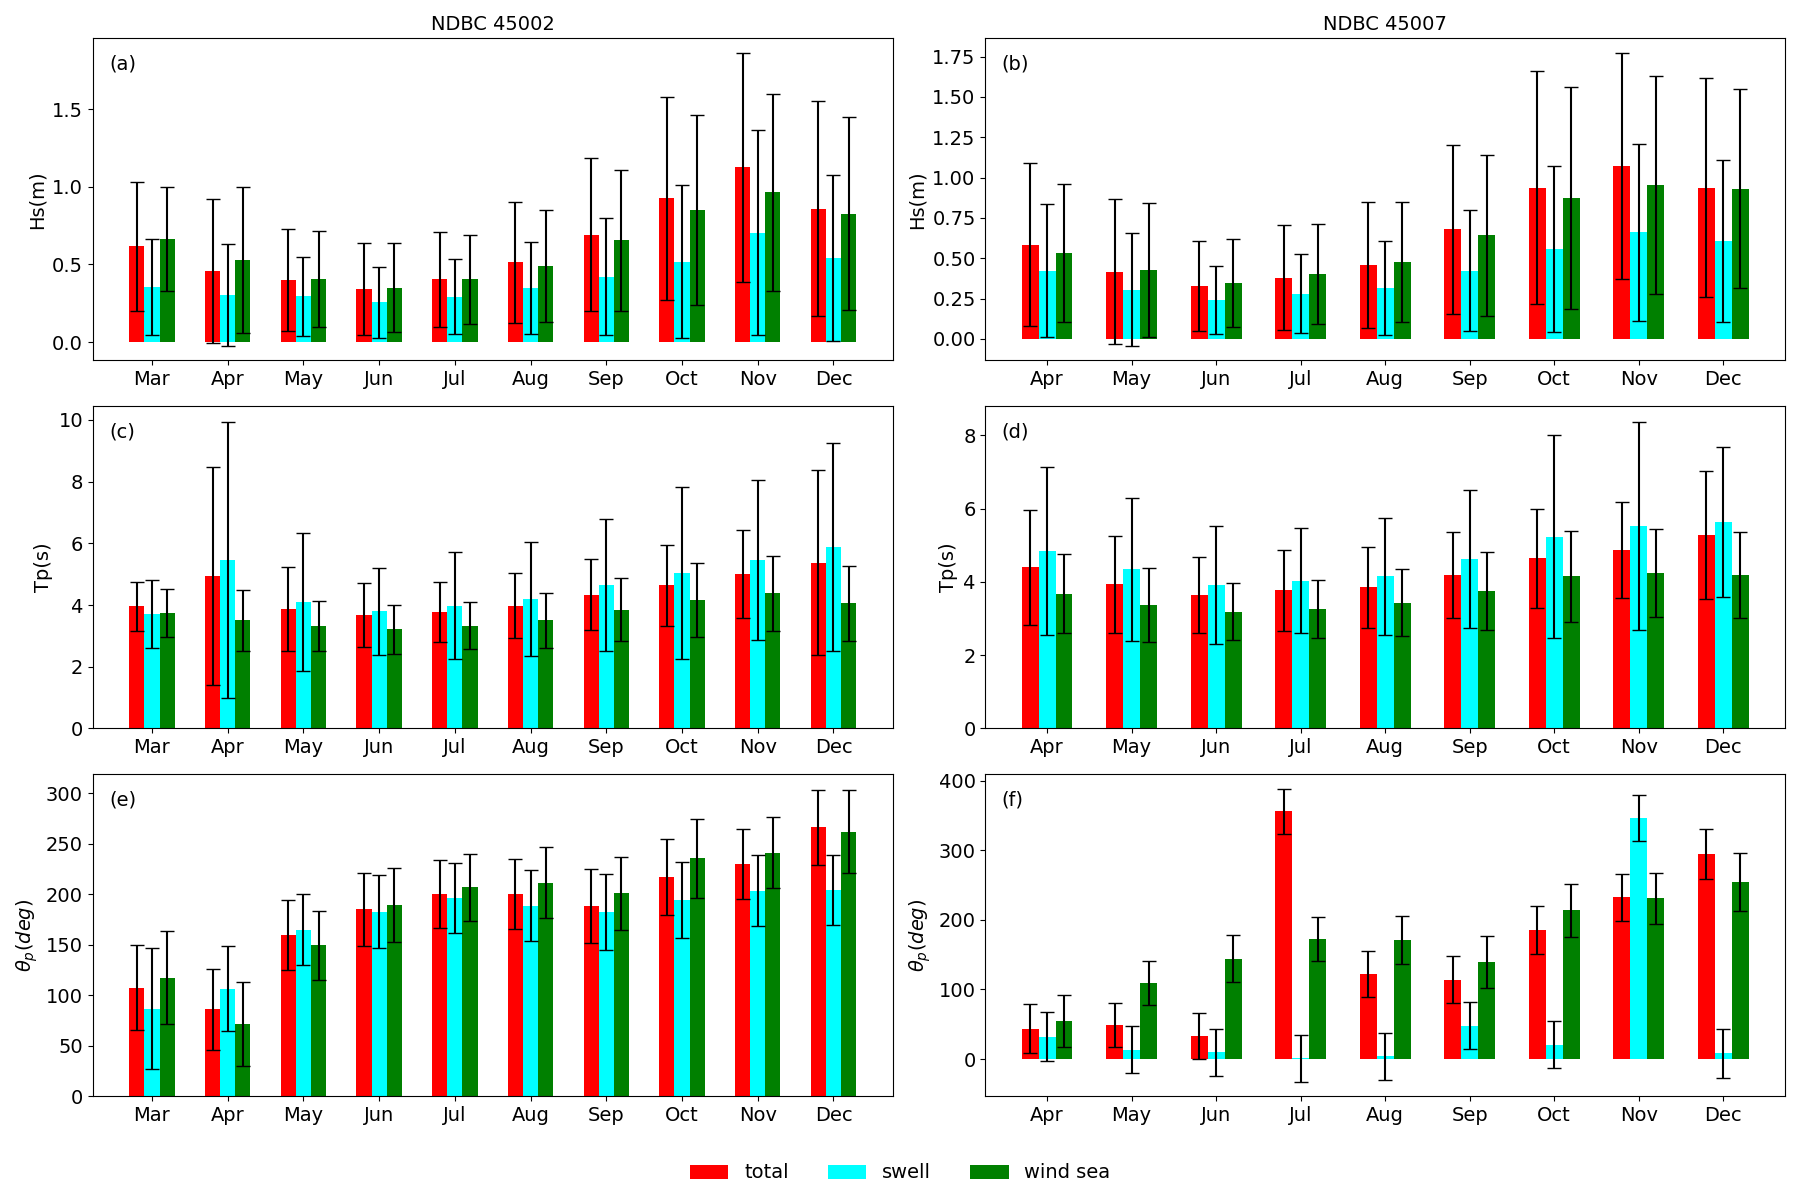
\includegraphics[width=1\textwidth]{chapter4/resources/ndbc_month.png}
  \caption{Monthly wave climates of NDBC stations 45002 and 45007, associated
  with each wave systems. (a-b) monthly total, swell, and windseda $H_s$ in 45002
  and 45007, respectively, (c-d) monthly total, swell, and windseda $T_p$ in
  45002 and 45007, respectively, (e-f) monthly total, swell, and windseda
  $\theta_p$ in 45002 and 45007, respectively }
  \label{fig:ndbc_month}
\end{figure}

Seasonal cycles reveal further contrasts between the two basins. At 45002, mean
$H_s$ is lowest in summer (June–July, ~0.3–0.5 m) and increases into autumn and
early winter, peaking in October–December when values often exceed 0.8 m (Figure
\ref{fig:ndbc_month}a). This increase is mainly driven by wind-sea, while swell
contributions remain secondary, underscoring the dominance of local storm
forcing in the north. Monthly $T_p$ values at 45002 (Figure
\ref{fig:ndbc_month}c) remain short throughout the year (~4–5 s for wind-sea,
~6–7 s for swell), with only modest winter lengthening. Wave directions
($\theta_p$; Figure \ref{fig:ndbc_month}e) are persistently southerly (180–220°)
in all months, reflecting the basin’s restricted geometry. By contrast, at
45007, summer months are again relatively calm ($H_s \approx 0.4$ m), but
October–December means often exceed 1.0 m, with both wind-sea and swell
contributing substantially (Figure \ref{fig:ndbc_month}b). Peak periods at 45007
lengthen in late autumn and winter, with swell $T_p$ frequently reaching 7–8 s
(Figure \ref{fig:ndbc_month}d), reflecting long-period wave propagation across
the full lake. Monthly directions (Figure \ref{fig:ndbc_month}f) confirm the
strongly bidirectional nature of the southern basin: southerly waves dominate in
spring and autumn, while northerly waves are frequent in summer and early
winter. Swell, in particular, alternates between north (~0–30°) and south
(~180–200°), highlighting the influence of opposing storm tracks and long-fetch
dynamics. Collectively, these seasonal patterns reinforce the interannual
findings: the northern basin remains consistently fetch-limited and southerly
dominated, while the southern basin experiences stronger seasonality, greater
energy, longer swell periods, and alternating bidirectional forcing.

\section{Discussions}
\label{c4_Discussions}

\subsection{Wave system in Lake Michigan nearshore regions}
\label{Wave system in Lake Michigan nearshore regions}

\begin{figure}[htbp]
  \centering
  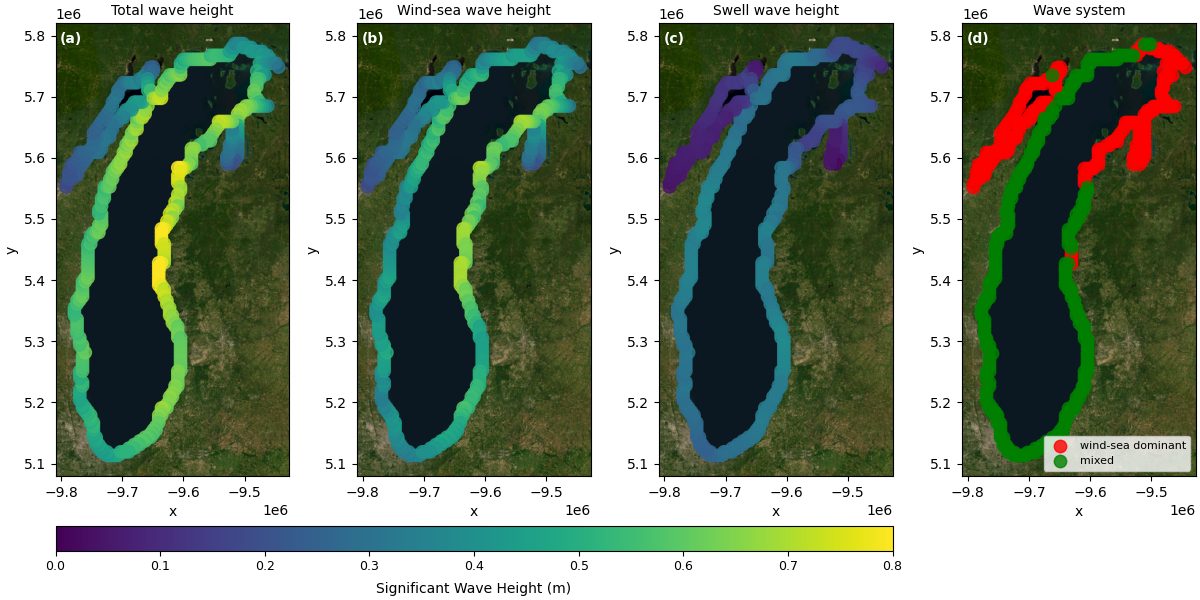
\includegraphics[width=1\textwidth]{chapter4/resources/nearshore_system_climate.png}
  \caption{Wave system (swell vs wind-sea vs total) in nearshore WIS stations in
  Lake Michigan. (a) significant wave height ($H_s$) for total wave system. (b)
  significant wave height ($H_s$) for wind-sea wave. (c) significant wave height
  ($H_s$) for swells. (d) Dominant conditions of wave system: red-windsea
  domiant, blue-swell dominant, green-mixed conditions. The blue does not
  present in the (d) as not nearshore stations are categorized as swell
  dominant.}
  \label{fig:nearshore_system}
\end{figure}

Wave systems in nearshore Wave Information Study stations of Lake Michigan were
presented in Figure \ref{fig:nearshore_system}. The wind-sea and swell data were
partitioned by Wave Information Study by WAM model configure. The total wave
height in Lake Michigan (Figure \ref{fig:nearshore_system}a) presented a clear
spatial variation that wave heights are higher in eastern shoreline than the
western shoreline due to strong south-eastern wind in the winter
\citep{huang_wave_2021}. The wind-sea waves share a similar spatial pattern with
the overall total waves (Figure \ref{fig:nearshore_system}b), where eastern
shoreline receieves larger waves than the western coastline. Compared to local
wind-sea waves, the swells (Figure \ref{fig:nearshore_system}c) distributed
uniformly accross the nearshore of Lake Michigan. The wave heights of swells
were relatively smaller than wind-sea as the most of wind-sea waves range
between 0.6-0.8 meters, while the swells span from 0.2-0.4 meters. Figure
\ref{fig:nearshore_system}d presented the relationship between these two wave
systems. In Lake Michigan, most of nearshore regions were classified into
mixed-conditions, where the ratio of wind-sea with total wave energy stay
between 0.25 to 0.75 (see Equation \ref{eq:eq4.10}). Noticed that in Green Bay
area (northwestern Lake Michigan) and Grand Traverse Bay (northeastern Lake
Michigan). The wave conditions are categorized as wind-sea dominant, indicating
that the swell impacts in these regions are relative tiny. The fetch fields in
these two bay areas are limited that the waves could not be grown completed into
swells. The spatial distributions of 

\subsection{Impact of wave system on coastal geomorphic change}
\label{Impact of wave system on coastal geomorphic change}

\begin{figure}[htbp]
  \centering
  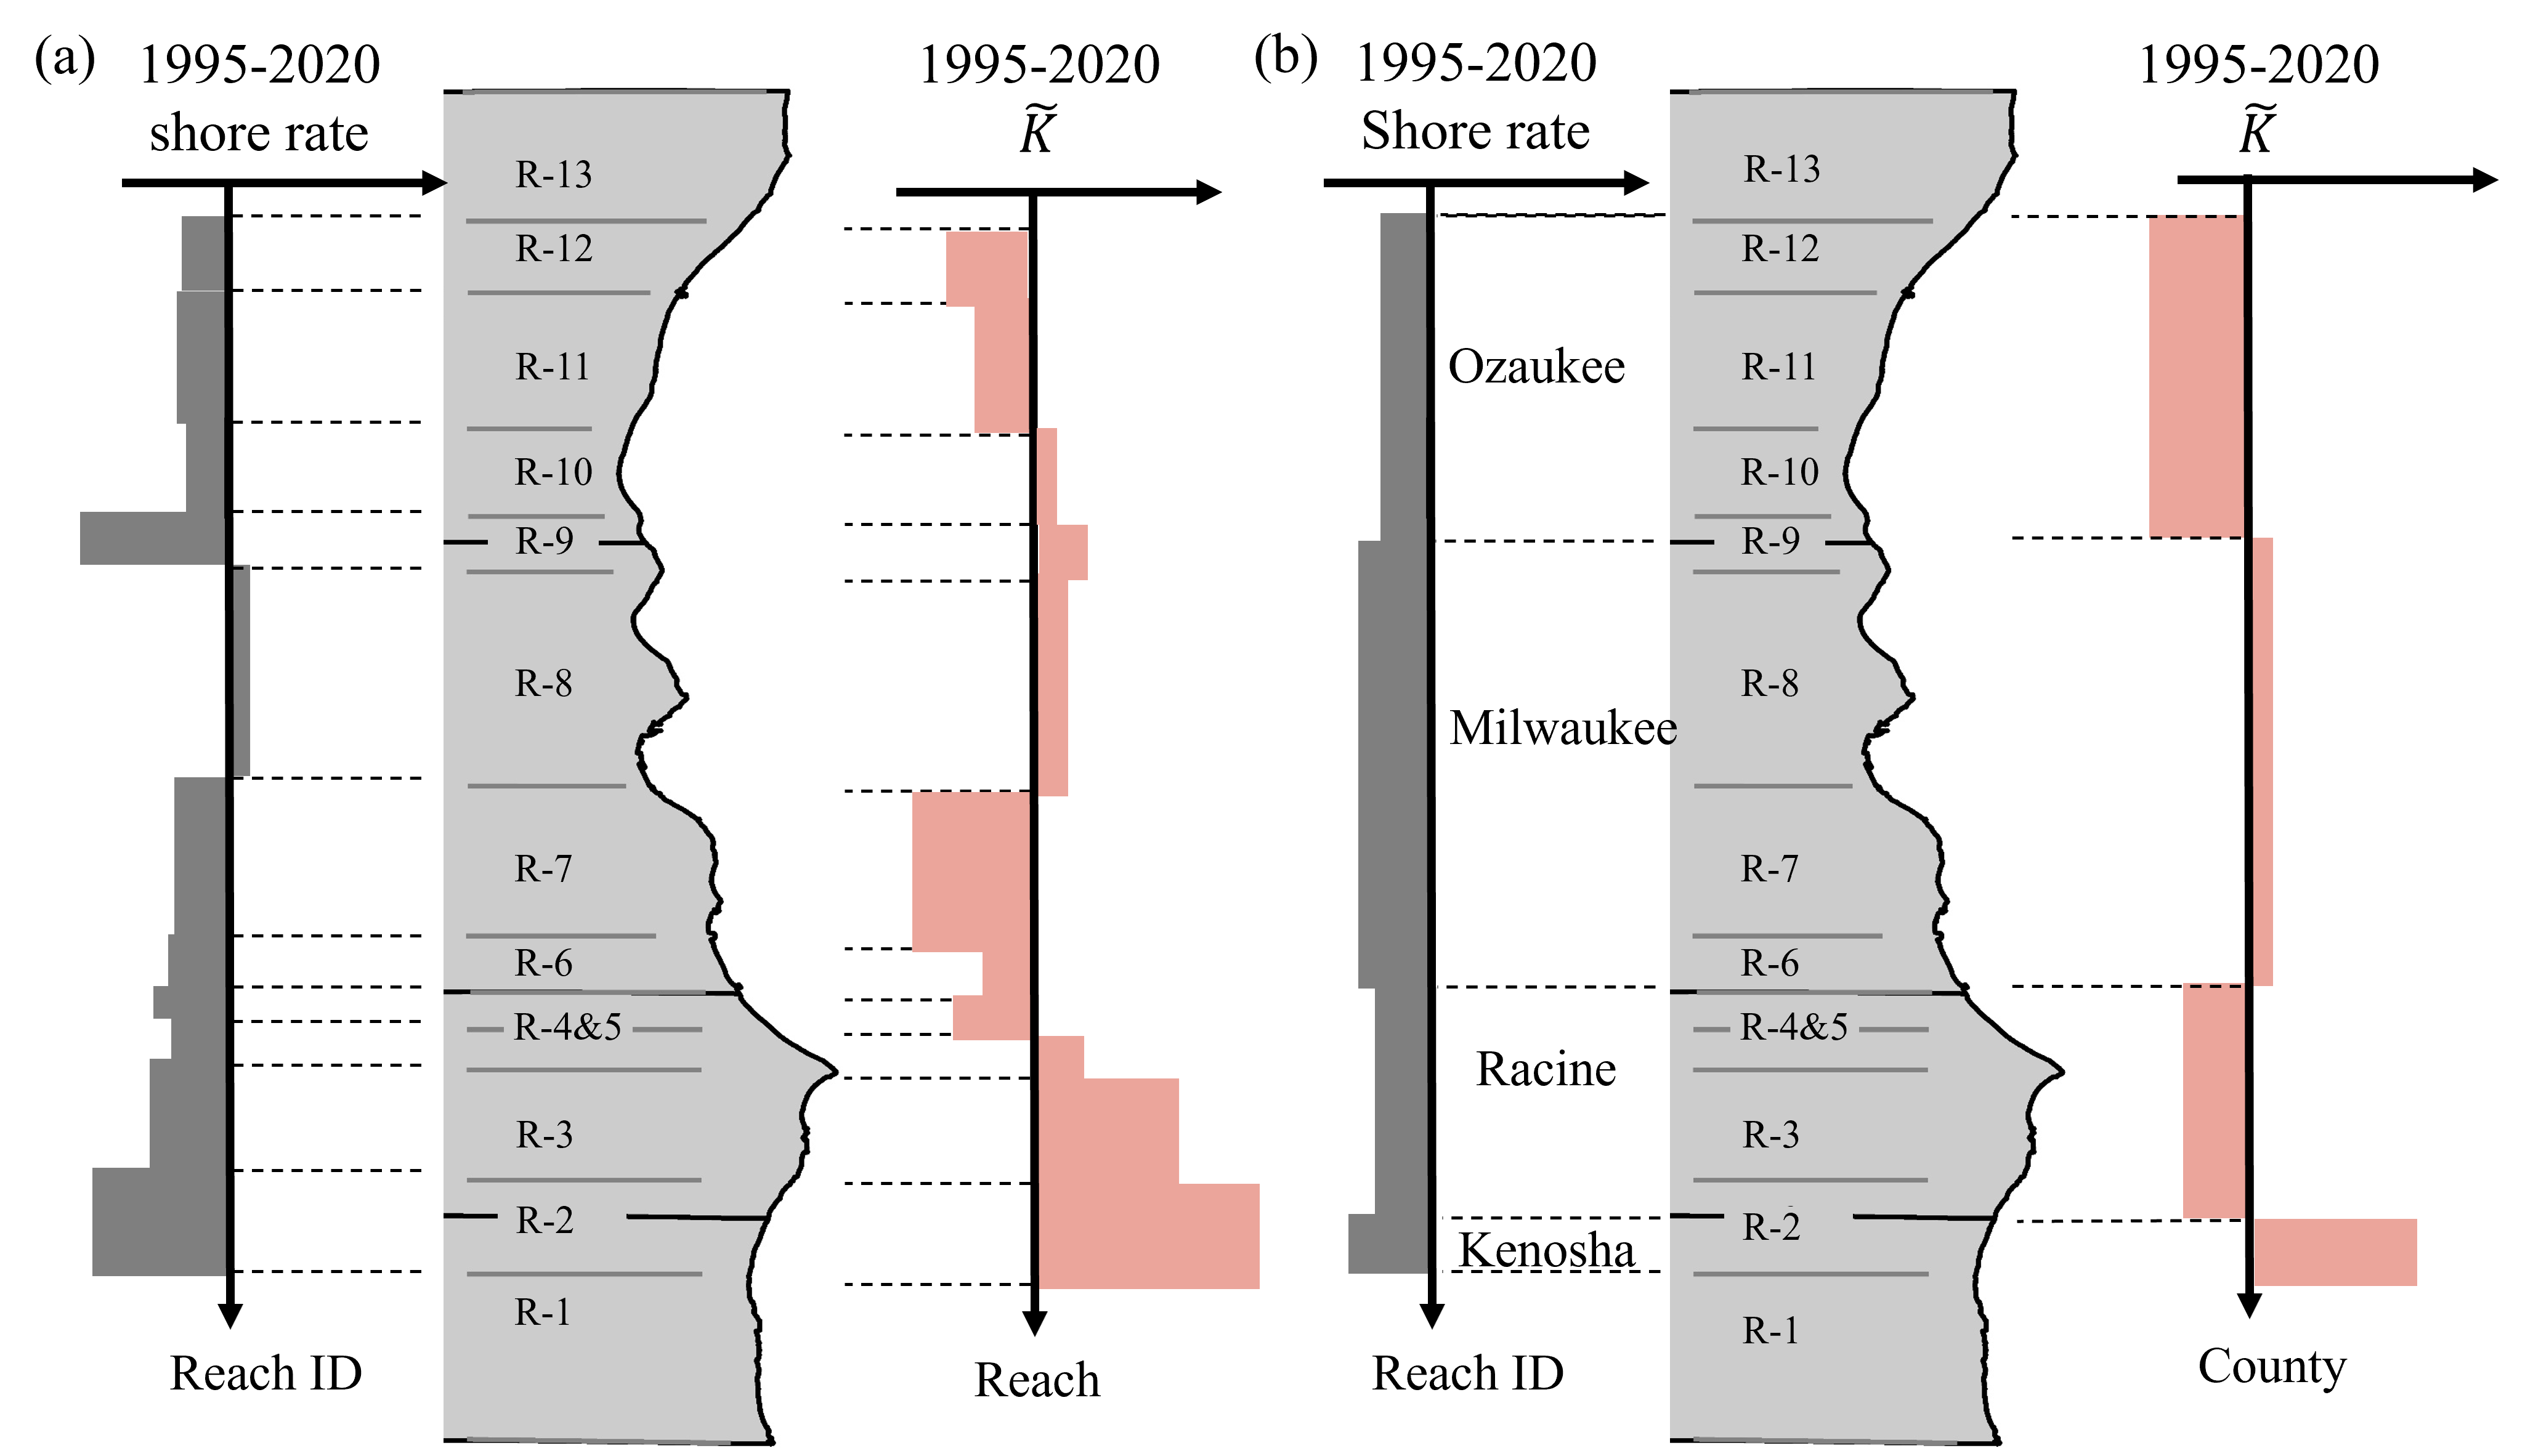
\includegraphics[width=1\textwidth]{chapter4/resources/nearshore_correlation.png}
  \caption{The shoreline erosion rate (1995-2020) vs wave system domiant
  coefficient $K$. Noticed that $\widetilde{K}$ is the standard-normalization of
  $K$ }
  \label{fig:nearshore_cor}
\end{figure}

Wave systems were known for its implications on oceanic subject, such as navigation,
habitats, etc. On the coastline, wave systems are also known as its impacts on coastal
geomorphology. The 

\subsection{Limitation}
\label{Limitation}

\section{Conclusion}
\label{c4_Conclusion}